\documentclass[
12pt,
a4paper,
final,
titlepage,
oneside,
]{report}

\usepackage[
    colorlinks=true,
    urlcolor=blue,
    filecolor=blue,
    linkcolor=red,
    bookmarks=true,
    citecolor=red,
]{hyperref}

%%%%%%%%%%%%%%%%%%%%%%%%%%%%%%%
%\usepackage{tocbibind}

%\usepackage{natbib}
%\bibliographystyle{plainnat}
%\setcitestyle{super,open={(},close={)}}%

\usepackage[hyperref=true, backend=bibtex, style=numeric, sorting=ynt]{biblatex}
%\bibliography{<database>}
%\bibliography{main}
\addbibresource{main.bib}
\DeclareCiteCommand{\citetitle}
  {\boolfalse{citetracker}%
   \boolfalse{pagetracker}%
   \usebibmacro{prenote}}
  {\ifciteindex
     {\indexfield{indextitle}}
     {}%
   \printtext[bibhyperref]{\printfield[citetitle]{labeltitle}}}
  {\multicitedelim}
  {\usebibmacro{postnote}}
%%%%%%%%%%%%%%%%%%%%%%%%%%%%%%%

\usepackage[frenchb]{babel}
\usepackage[utf8]{inputenc}
\usepackage{courier}
\usepackage{csquotes}
\usepackage[titles]{tocloft}
\usepackage{enumitem}
\usepackage{datetime}
\usepackage{float}
\usepackage{pdfpages}
\usepackage{nameref}
\usepackage{setspace}
\usepackage{import}
\usepackage[pagestyles]{titlesec}
\usepackage[T1]{fontenc}
\usepackage{fancyhdr}
\usepackage[
    titletoc,
    header,
    title
]{appendix}
\usepackage[
    font=footnotesize,
    labelfont=
    {
        sf,
        bf
    },
    margin=1cm
]{caption}
\usepackage{listings}
\usepackage{bold-extra}
\usepackage[
    top=3cm,
    bottom=3cm,
    left=2cm,
    right=2cm,
    headheight=2cm,
    headsep=1cm,
    footskip=2cm
]{geometry}
\usepackage[
    activate={true,nocompatibility},
    final,
    tracking=true,
    kerning=true,
    spacing=true,
    factor=1100,
    stretch=10,
    shrink=10
]{microtype}
\microtypecontext{spacing=nonfrench}
\usepackage{cleveref}
\usepackage{booktabs}
\usepackage{tabularx}

\newcolumntype{R}{>{\raggedleft\arraybackslash}X|}
%
\usepackage{array} 
\usepackage{graphicx}
\graphicspath{ {images/} }

% Nagger ------------------------------------------------------------------------------------
\RequirePackage[l2tabu, orthodox]{nag}
% Sets doc-wide fonts -----------------------------------------------------------------------
\renewcommand*\familydefault{\ttdefault}
% Setup caption for listings ----------------------------------------------------------------
%\captionsetup[lstlisting]{font={small,tt}}
\captionsetup{font={scriptsize, tt}, labelfont={sc, it},textfont={it, sc}}
% Fuzz --------------------------------------------------------------------
\hfuzz20pt % Don't bother to report over-full boxes if over-edge is < 2pt
% includes ----------------------------------------------------------------------------------
%\usepackage[many]{tcolorbox}

\newtcolorbox[auto counter, crefname={Note}{Notes}]{notebox}{
freelance,
colback=white,
frame code={},
interior titled code={
  \fill[rounded corners=8pt,gray!30!gray]
    (title.south west) --
    (title.south) --
    ([yshift=20pt]title.south) --
    ([yshift=20pt,xshift=4cm]title.south) --
    ([xshift=4cm]title.south) --
    (title.south east) {[sharp corners] --
    ([yshift=-6pt]title.south east) --
    ([yshift=-6pt]title.south west) } -- cycle;
  \draw[rounded corners=8pt,gray,line width=1pt]
    (title.west|-frame.south west) --
    (title.south west) --
    (title.south) --
    ([yshift=20pt]title.south) --
    ([yshift=20pt,xshift=4cm]title.south) --
    ([xshift=4cm]title.south) --
    (title.south east) --
    (title.east|-frame.south east) --
    cycle;
  \node at ([xshift=2cm,yshift=10pt,anchor=south]title.south)
    {\ttfamily Addendum};
  },
title={\mbox{}},
top=12pt,
fontupper=\ttfamily,
oversize=-2cm,
before={\vskip24pt\par\noindent},
after={\par\vskip12pt},
box align=center
} 
%% tikz --------------------------------------------------------------------------
%\usepackage{tikz}
%\usepackage{varwidth}
%\usetikzlibrary{calc}
%\newcommand{\customcolorbox}[4][\textwidth-\pgfkeysvalueof{/pgf/inner xsep}-2mm]{%
%\begin{figure}[!h]
%    \centering
%    \begin{tikzpicture}
%        \node[line width=.5mm, rounded corners, draw=#2, inner ysep=10pt, text width=#1, outer sep=0] (one) {\vspace*{15pt}\\\begin{varwidth}{\textwidth}#4\end{varwidth}};
%        \node[text=white,anchor=north east,align=center, minimum height=20pt] (two) at (one.north east) {\textbf{#3} \hspace*{0.5mm}};
%        \path[fill=#2]
%            (one.north west|-two.west) --
%            ($(two.west)+(-1.5cm,0)$)
%            to[out=0,in=180] (two.south west) --
%            (two.south east) [rounded corners] --
%            (one.north east) --
%            (one.north west) [sharp corners] -- cycle;
%        \node[text=white,anchor=north east,align=center, minimum height=20pt, text height=2ex] (three) at (one.north east) {\textbf{#3} \hspace*{.5mm}};
%    \end{tikzpicture}
%\end{figure}
%}
\usepackage[many]{tcolorbox}

\newcommand{\custombox}[2]{
	\begin{tcolorbox}%
	[%
		box align=center,
		colframe=gray!10!#1,%
		boxrule=1pt,%
		leftrule=3mm,%
		colback=#1!20!white%
	]%
	#2%
	\end{tcolorbox}%
}

\newcommand{\important}[1]{\custombox{red}{#1}}

\newcommand{\useful}[1]{\custombox{blue}{#1}}

\newcommand{\remark}[1]{\custombox{gray}{#1}}

\newcommand{\note}[1]{%
	\begin{tcolorbox}%
	[%
		box align=center,
		colback=gray!5!white,%
		colframe=gray!75!black,%
		fonttitle=\bfseries,%
		colbacktitle=gray!85!black,%
		enhanced,%
		attach boxed title to top center={yshift=-2mm},%
		title=Note%
	]%
	#1%
	\end{tcolorbox}%
}
% Chapter title formatting ----------------------------------------------
\titleformat
{\chapter} % command
[block] % shape
{\bfseries\Huge} % format
{\thechapter.} % label
{1em} % sep
{
%    \rule{\textwidth}{1pt}
    \vspace{1ex}
%    \centering
} % before-code
[
\vspace{-0.5ex}%
%\rule{\textwidth}{0.3pt}
] % after-code

\titlespacing*{\chapter}{0pt}{-50pt}{40pt}

% Section title formatting ----------------------------------------------
\titleformat{\section}[block]
{\Large\bfseries}
{\thesection.}{0.5em}{}

% Subsection title formatting -------------------------------------------
\titleformat{\subsection}[block]
{\large\bfseries}
{\thesubsection.}{0.5em}{}

% Subsection title formatting -------------------------------------------
\titleformat{\subsubsection}[block]
{\large\bfseries}
{\thesubsubsection.}{0.5em}{}

% Define dots in TOC ----------------------------------------------------------
\renewcommand{\cftpartleader}{\cftdotfill{\cftdotsep}} % for parts
\renewcommand{\cftchapleader}{\cftdotfill{\cftdotsep}} % for chapters
\renewcommand{\cftsecleader}{\cftdotfill{\cftdotsep}}


% Set space between paragraphs -----------------------------------------------------
\setlength{\parskip}{1em}

% Depth of section numbering ----------------------
\setcounter{secnumdepth}{4}

% Format of tables -----------------------------------------------------------------
\setlength\cftbeforechapskip{20pt}
\renewcommand\cftfigafterpnum{\vskip5pt\par}
\renewcommand\cfttabafterpnum{\vskip5pt\par}
\setlength{\cftfignumwidth}{4em}  % Modify number width in LoF
\setlength{\cfttabnumwidth}{4em}
\setlength{\cftchapnumwidth}{2em}
\setlength{\cftsecnumwidth}{3em}
\setlength{\cftsubsecnumwidth}{4em}
% Define links ----------------------------------------------------------------
\newcommand{\jplink}{https://www.google.com/url?q=https://fas.org/irp/doddir/dod/jp3_09_3.pdf\&sa=D\&ust=1457816834668000\&usg=AFQjCNEpTH7xDsiu3EjM3xcSy5AatewYrA}
\newcommand{\onethreetwolink}{http://www.132virtualwing.org/}
\newcommand{\thirdwinglink}{http://http://www.3rd-wing.net/}
\newcommand{\dcslink}{http://www.digitalcombatsimulator.com/en/}
% Define constants -------------------------------------------------------------
\newcommand{\version}{DRAFT 1}
\newcommand{\rgt}{319th Rgt}
\newcommand{\thirdwing}{\href{\thirdwinglink}{3rd Wing}}
\newcommand{\jp}{\href{\jplink}{JP3-09.3}}
\newcommand{\onethreetwo}{\href{\onethreetwolink}{132nd vWing}}
\newcommand{\docname}{``319th Rgt - Close Air Support - Manuel du pilote''}
\newcommand{\dcs}{\href{\dcslink}{Digital Combat Simulator}}
\newcommand{\inmem}{``In Memoriam Flying Manu''}
\newcommand{\ttitle}{Close Air Support - Manuel du pilote}
\newcommand{\footer}{\rgt{} - \ttitle{} - \version{}}
% Long enum
\newlist{longenum}{enumerate}{8}
\setlistdepth{8}
\setlist[longenum,1]{label=\roman*)}
\setlist[longenum,2]{label=\alph*)}
\setlist[longenum,3]{label=\arabic*)}
\setlist[longenum,4]{label=(\roman*)}
\setlist[longenum,5]{label=(\alph*)}
\setlist[longenum,6]{label=(\alph*)}
\setlist[longenum,7]{label=(\alph*)}
\setlist[longenum,8]{label=(\alph*)}

%%%%%%%%%%%%%%%%%%%%%%%%%%%%%%%%%%%%%%%%%%%%%%%%%%%%%%%%%%%%%%%%%%%%%%%%%%%%%%%%%
% Define commands for enumeration
\newcommand{\e}{\begin{longenum}[label*={\alph*}., topsep=1em,itemsep=1em,partopsep=1em,parsep=1em, labelsep=1em, leftmargin=2em]}

\newcommand{\ee}{\begin{longenum}[label*={\arabic*}, topsep=1em,itemsep=1em,partopsep=1em,parsep=1em, labelsep=1em, leftmargin=2em]}

\newcommand{\eee}{\begin{longenum}[label*=({\alph*}), topsep=1em,itemsep=1em,partopsep=1em,parsep=1em, labelsep=1em, leftmargin=2em]}

\newcommand{\eeee}{\begin{longenum}[label=({\arabic*}), topsep=1em,itemsep=1em,partopsep=1em,parsep=1em, labelsep=1em, leftmargin=2em]}

\newcommand{\eeeee}{\begin{longenum}[label={\Roman*}., topsep=1em,itemsep=1em,partopsep=1em,parsep=1em, labelsep=1em, leftmargin=2em, before*=\small, font=\small]}

\newcommand{\eeeeee}{\begin{longenum}[label*=({\roman*}), topsep=1em,itemsep=1em,partopsep=1em,parsep=1em, labelsep=1em, leftmargin=2em, before*=\small, font=\small]}

\newcommand{\eeeeeee}{\begin{longenum}[label*=({\arabic*}), topsep=0em,itemsep=1em,partopsep=0em,parsep=0em, labelsep=1em, leftmargin=2em, before*=\footnotesize, font=\footnotesize]}


% resume
\newcommand{\re}{\begin{longenum}[resume, label*={\alph*}., topsep=1em,itemsep=1em,partopsep=1em,parsep=1em, labelsep=1em, leftmargin=3em]}
\newcommand{\ree}{\begin{longenum}[resume, label*={\arabic*}, topsep=1em,itemsep=1em,partopsep=1em,parsep=1em, labelsep=1em, leftmargin=4em]}
\newcommand{\reee}{\begin{longenum}[resume, label*=({\alph*}), topsep=1em,itemsep=1em,partopsep=1em,parsep=1em, labelsep=1em, leftmargin=5em]}
\newcommand{\reeee}{\begin{longenum}[resume, label*=({\arabic*}), topsep=1em,itemsep=1em,partopsep=1em,parsep=1em, labelsep=1em, leftmargin=6em]}
\newcommand{\reeeee}{\begin{longenum}[resume, label*={\Roman*}., topsep=1em,itemsep=1em,partopsep=1em,parsep=1em, labelsep=1em, leftmargin=3em]}
\newcommand{\reeeeee}{\begin{longenum}[resume, label*=({\roman*}), topsep=1em,itemsep=1em,partopsep=1em,parsep=1em, labelsep=1em, leftmargin=3em]}

% terminate
\newcommand{\ed}{\end{longenum}}
%%%%%%%%%%%%%%%%%%%%%%%%%%%%%%%%%%%%%%%%%%%%%%%%%%%%%%%%%%%%%%%%%%%%%%%%%%%%%%%%%

% Title item
\newcommand{\itemt}[2]{\item #1\\[2ex]#2}

% Define default styles ------------------------------------------------------------
\newcommand{\deflhead}{\minipage[b]{.7\linewidth}\leftmark\endminipage}
\newcommand{\defrhead}{
\includegraphics[width=1cm]{images/319th.png}}
\newcommand{\deflfoot}{\footnotesize \footer}
\newcommand{\defrfoot}{\thepage}
% -----------------------------------------------------------------------------------
\fancypagestyle{default}{%
  \fancyhf{}% Clear header and footer
  \fancyhead[L]{\deflhead{}}
  \fancyhead[R]{\defrhead{}}
  \fancyfoot[L]{\deflfoot{}}% Custom footer
  \fancyfoot[R]{\defrfoot{}}% Custom footer
  \renewcommand{\headrulewidth}{0.4pt}% Line at the header visible
  \renewcommand{\footrulewidth}{0.4pt}% Line at the footer visible
}

% Redefine the plain page style
\fancypagestyle{plain}{%
  \fancyhf{}% Clear header and footer
  \fancyhead[L]{\deflhead{}}
  \fancyhead[R]{\defrhead{}}
  \fancyfoot[L]{\deflfoot{}}% Custom footer
  \fancyfoot[R]{\defrfoot{}}% Custom footer
  \renewcommand{\headrulewidth}{0.4pt}% Line at the header visible
  \renewcommand{\footrulewidth}{0.4pt}% Line at the footer visible
}
\pagestyle{default}
\newcommand{\colorboxred}{red!40!gray}
\newcommand{\colorboxgreen}{green!40!gray}
\newcommand{\colorboxblue}{blue!40!gray}
\lstset{
  frame=left, frame=bottom,
  extendedchars=false,
  escapeinside="",
  numbers=left,
  basicstyle=\small\normalfont\sffamily,    % the size of the fonts that are used for the code
  stepnumber=1,                           % the step between two line-numbers. If it is 1 each line will be numbered
  numbersep=0cm,                          % how far the line-numbers are from the code
  tabsize=2,                              % tab size in blank spaces
  extendedchars=true,                     %
  breaklines=true,                        % sets automatic line breaking
  captionpos=b,                           % sets the caption-position to top
  mathescape=true,
  %stringstyle=\color{white}\ttfamily,
  showspaces=false,
  showtabs=false,
  xleftmargin=5pt,
  xrightmargin=5pt,
  framexleftmargin=5pt,
  framexrightmargin=5pt,
  framexbottommargin=5pt,
  framextopmargin=5pt,
  showstringspaces=false
 }
\newcommand{\efig}[2]{
	\begin{figure}[H]
	    \includegraphics[width=\textwidth]{#1.png}
	    \caption{#2}
	    \label{#1}
	\end{figure}
}

%\newcommand{\epdf}[3]{
%	\begin{figure}
%		\centering 
%		\includepdf[addtolist={1, figure , #2 , #1 }, pages=#3]{./images/#1.pdf}
%	\end{figure}
%}

	

\usepackage[acronym,toc]{glossaries}
% command: makeglossaries %
\makeglossaries

\newcommand{\newgls}[4]{% 1: abbrev 2: full name 3: ref 4: desc
	\newglossaryentry{#3g}{%
		name={#1},%
		description={#4}%
	}%
	\newglossaryentry{#3}{%
		type=\acronymtype,%
		name={#1},%
		description={#2},%
		first={#2 (#1)\glsadd{#3g}},%
		see=[Explication:]{#3g}%
	}%
}

\newgls{FFA}{Free Fire Area}{ffa}{%
Une zone spécifique dans laquelle le tir est autorisé sans coordination préalable
}

\newgls{FSCL}{Fire Support Coordination Line}{fscl}{%
Mesure de coordination du tir mise en place par le \gls{gc} au sein d'une zone d'opération; tout tir au delà de cette ligne doit être préalablement coordonné avec le \gls{gc} local, et avant laquelle tout tir doit être coordonnée avec le \gls{gc} qui a établi la FSCL
}

\newgls{CFL}{Coordinated Firing Line}{cfl}{%
Ligne au delà de laquelle le tir est autorisé sans coordination avec l'échelon supérieur
}

\newgls{NAI}{Named Area of Interest}{nai}{%
Zone particulière à laquelle on aura attribué un nom (ou qui porte déjà un nom, par ex. une ville)
}

\newgls{TAI}{Target Area of Interest}{tai}{%
Zone cible particulière
}

\newgls{AOF}{Azimuth Of Fire}{aof}{%
Direction dans laquelle tire une unité
}

\newgls{IFF}{Identitification Friend or Foe}{iff}{%
Système électronique embarqué permettant d'interroger à distance un appareil et de l'identifier comme ami
}

\newgls{PID}{Positive Identification}{pid}{%
Identification visuelle, électronique, \gls{iff} ou autre obtenue par l'observation et l'analyse des caractéristiques de la cible
}

\newgls{CP}{Contact Point}{cp}{%
Point sur lequel, lorsqu'elle arrive dessus, une unité est censée en contacter une autre
}

\newgls{POF}{Priorities Of Fire}{pof}{%
Priorités de tir
}

\newgls{COE}{Concept Of Employment}{coe}{%
Façon d'employer quelque chose
}

\newgls{JIPOE}{Joint Intelligence Preparation of the Operational Environment}{jipoe}{%
Le processus analytique par lequel les organisations de renseignement produisent des estimations et autres pour aider au processus de prise de décision pas le \gls{jfc}
}

\newgls{CAS request}{CAS request}{req}{%
Une requête \gls{cas} est une demande de \gls{cas} émise par une unité alliée au sol pour obtenir un support aérien. Ce support peut être planifié à l'avance (``Pre-planned \gls{cas}''), ou immédiat (``On-call \gls{cas}'')
}

\newgls{OPLAN}{Operational Plan}{oplan}{%
\parbox{\linewidth}{1. Tout plan pour la conduite d'une opération militaire préparée en réponse à une situation effective ou prévue.}\glvs{}
\parbox{\linewidth}{2. Un plan Joint complet et détaillé contenant la description complète du \gls{conops}, toutes les annexes d'application au plan, et une chronologie prévue de l'emploi de la force et du déploiement}
}

\newgls{TOS}{Time On Station}{tos}{%
Heure d'arrivée prévue sur la zone cible, de patrouille, sur l'objectif, etc.
}

\newgls{ACM}{Airspace Control Measure}{acm}{%
Directive visant à rendre l'utilisation des unités aériennes efficaces et aptes à remplir leur mission tout permettant le transit sécurisé dans l'espace aérien
}

\newgls{ACA}{Airspace Coordination Area}{aca}{%
Un bloc tridimensionnel d'espace aérien se trouvant dans une zone cible, défini par l'autorité appropriée, dans lequel les appareils alliés sont normalement hors de danger d'être touché par un tir ami provenant du sol (artillerie, principalement, ou Kakane, parfois)
}


\newgls{DAS}{Deep Air Support}{das}{%
Le DAS englobe le \gls{ai}, le \gls{ar} et le \gls{scar}, trois types de missions qui, à l'inverse du \gls{cas}, sont dirigées contre les unités ennemies au sol qui ne trouvent pas à proximité des forces au sol alliées
}

\newgls{AI}{Air Interdiction}{ai}{%
\parbox{\linewidth}{L'interdiction aérienne consiste à utiliser une unité aérienne pour attaquer des cibles ennemies tactiques au sol qui ne trouvent pas à proximité de forces au sol alliées}\glvs{}
\parbox{\linewidth}{L'interdiction diffère du \gls{cas} en cela qu'elle ne soutient pas directement les opérations des forces au sol, et qu'elle n'est pas coordonnée aussi étroitement avec ces dernières}\glvs{}
\parbox{\linewidth}{A la différence du bombardement stratégique, l'interdiction n'est pas une campagne aérienne à part entière, de par son objectif ultime qui reste le soutien des forces au sol alliées, là où le bombardement stratégique vise à défaire l'ennemi par la puissance aérienne uniquement}\glvs{}
\parbox{\linewidth}{L'objectif de l'interdiction est de retarder, perturber ou détruire les forces ennemies ou la logistique en route vers la zone de combat avant qu'elles en deviennent un facteur pour les forces alliées. Même à ce degré, une distinction est faite entre l'interdiction stratégique et l'interdiction tactique; l'interdiction stratégique est prévue à grande échelle et sur le long terme, là où l'interdiction tactique agit de manière rapide et localisée}
}

\newgls{SCAR}{Air Interdiction}{scar}{%
\glvs{}
\parbox{\linewidth}{Le SCAR est une mission dont l'objectif est l'acquisition et le rapportage de cible pour le \gls{das}. Les missions SCAR coordonnent et peuvent marquer les cibles pour les missions \gls{ai}, ou repérer précisément les cibles pour les missions \gls{ar}. Le SCAR ne doit pas être confondu avec le \gls{faca}}\glvs{}
\parbox{\linewidth}{\gle
	\item Le SCAR ne nécessite pas une qualification \gls{faca} pour le \gls{tac} des missions \gls{das}
	\item Le SCAR fournit des cibles, des positions, des descriptions, des informations quant à la météo ou la menace
	\item Le SCAR peut fournir la marque mais pas l'autorisation de tir
	\item Le SCAR confirme ou découvre des menaces air-sol
	\item Le SCAR assiste à l'établissement de la \gls{bda}
	\item Le SCAR diffère d'une mission de reconnaissance de par le fait qu'il découvre les cibles et coordonne leurs destruction, et qu'il sera typiquement armé et équipé de manière à améliorer la désignation des cibles
\gled}\glvs{}
\parbox{\linewidth}{Le SCAR est particulièrement utile dans un environnement riche en cible. Un appareil en mission SCAR qui se trouve à court de munitions peut continuer sa mission}
}

\newgls{AR}{Armed Reconnaissance}{ar}{%
\parbox{\linewidth}{La reconnaissance armée est utilisée quand la position exacte de la cible est inconnue, et que le pilote devra localiser et engager les cibles potentielles pour accomplir l'objectif. Ces missions impliquent que l'appareil sera exposé pendant de longues période en territoire ennemi, à la recherche de cibles potentielles}\glvs{}
\parbox{\linewidth}{\gle
	\item Identifier des cibles dont la position est inconnue et les engager avant qu'elles ne deviennent un facteur
	\item Empêcher l'ennemi d'effectuer un mouvement non détecté ou d'accéder à une zone clef
	\item Fournir un avertissement précoce quant à la position et aux intentions de l'ennemi
	\item Empêcher ou dégrader la mobilité de l'ennemi
	\item Reconnaître une grande étendue de terrain qui serait moins facilement explorée par les forces au sol amies
	\item Attaquer des cibles dont la destruction doit se faire rapidement (menaces en mouvement vers le front, par exemple)
	\item Soutien lors des opérations de sécurité, soit comme unité de soutien du support ou comme couverture, garde ou écran principal
\gled}
}

\newgls{BAI}{Battlefield Air Interdiction}{bai}{%
Cfr AI
}

\newgls{COMSEC}{Communications Security}{comsec}{%
Tout ce qui a trait à la sécurisation des communications alliées
}

\newgls{FSCM}{Fire Support Coordination Measure}{fscm}{%
Directive mise en place pour coordonner le tir de support (artillerie)
}

\newgls{FSCOORD}{Fire Support Coordinator}{fscoord}{%
Officier en charge de la coordination du tir de support (artillerie)
}

\newgls{COA}{Course Of Action}{coa}{%
Ligne de conduite, façon de faire
}

\newgls{5-Line}{5-Line}{5l}{%
La 5-Line est une version résumée de la \gls{9l}, réservée aux hélicoptères, et centrées sur les forces alliées
}

\newgls{9-Line}{9-Line}{9l}{%
Format standard du briefing donné par le J-TAC/FAC(A)
}

\newgls{FLOT}{Forward Line Of Troops}{flot}{%
Ligne de front, là où les troupes alliées sont les plus avancées
}

\newgls{FRAGO}{Fragmentary Order}{frago}{%
Forme abrégée de l'\gls{opord} publiée journellement
}

\newgls{BOC}{Bombs On Coordinates}{boc}{%
Méthode d'attaque consistant à attaquer la cible au moyen d'une munition intelligente sur des coordonnées, parfois sans jamais acquérir la cible. La méthode d'attaque BOC implique de rentrer \textbf{directement} les coordonnées de la cible dans le système lors du \gls{cas} brief, et d'effectuer le read-back de la ligne 6 en \textbf{relisant les coordonnées entrées dans le système}
}

\newgls{HMCS}{Helmet Mounted Cueing System}{hmcs}{%
Système de visée monté sur le casque (HMS)
}

\newgls{FLIR}{Forward Looking Infrared}{flir}{%
Équipement embarqué permettant de voir en infrarouge devant l'appareil
}

\newgls{FOV}{Field Of View}{fov}{%
Champ de vision
}

\newgls{IDF}{Indirect Fire}{idf}{%
Feu indirect, c-à-d artillerie
}

\newgls{TRP}{Target Reference Point}{trp}{%
Point de référence cible (NAV TGT dans le PVI800)
}

\newgls{BOT}{Bombs On Target}{bot}{%
Méthode d'attaque consistant à attaquer après l'avoir acquise visuellement ou via les senseurs embarqués
}

\newgls{stack}{stack}{stack}{%
Mise en attente des appareils de manière sécurisée
}

\newgls{GPS}{Global Positionning System}{gps}{%
Système permettant d'obtenir les coordonnées d'un point sur la terre au moyen d'une constellation de satellites
}

\newgls{LRF}{Laser Range Finder}{lrf}{%
Laser servant à calculer une distance
}

\newgls{JDAM}{Joint Direct Attack Munition}{jdam}{%
Un JDAM est un kit qui convertit une bombe lisse en bombe guidée \gls{gps}
}

\newgls{MSL}{Mean Sea Level}{msl}{%
Niveau moyen de la mer
}

\newgls{HVT}{High Value Target}{hvt}{%
Cible de grande importance
}

\newgls{CSAR}{Combat Search and Rescue}{csar}{%
Recherche et sauvetage de combat
}

\newgls{OPCON}{Operationnal Control}{opcon}{%
Entité qui exerce le contrôle opérationnel (stratégique), par opposition au contrôle tactique (\gls{tacon})
}

\newgls{SEAD}{Suppression of Ennemy Air Defence}{sead}{%
Aussi appelé ``Wild Weasel'', ou ``Iron Hand''. Action visant à neutraliser les défenses anti-aériennes ennemies, pas uniquement les \glspl{sam} ou \glspl{aaa}, mais également les \glspl{ewr} et le \gls{ccc}. Cette action peut être effectuée au moyen d'armement, ou de moyens de guerre électronique
}

\newgls{CID}{Combat Identification}{cid}{%
Capacité de différencier les cibles potentielles, mobiles ou fixes, dans de grandes zones, comme amies, ennemies ou neutre, dans un temps très court, avec un grand degré de certitude, et à la distance suffisante, pour permettre les décisions d'emploi de la force
}

\newgls{AOD}{Air Operation Directive}{aod}{%
Directive émise par le \gls{jfacc} concernant la conduite des opération aériennes%
}

\newgls{ROE}{Rule of Engagement}{roe}{%
Décrit les circonstances, les conditions, la manière et la proportion dans lesquelles l'usage de la force est autorisé%
}

\newgls{TGO}{Terminal Guidance Operation}{tgo}{%
Action de fournir aux appareils ou aux armes des informations supplémentaires relatives à la cible par la voix, l'électronique, les communications visuelles ou des moyens mécaniques%
}

\newgls{TAC}{Terminal Attack Control}{tac}{%
Autorité qui contrôle la manœuvre %
}

\newgls{BDA}{Battle Damage Assessment}{bda}{%
Évaluation des dégâts infligés à la cible, ou aux cibles, suite à un engagement%
}

\newgls{FAC(A)}{Forward Air Controller}{faca}{%
Un pilote spécialement qualifié qui contrôle, depuis les airs, d'autres appareils engagés en opération de \gls{cas}%
}

\newgls{J-TAC}{Joint Terminal Attack Controller}{jtac}{%
Un membre du personnel qualifié qui contrôle, depuis une position au sol avancée, les appareils engagés en opération de CAS ou d'autres types d'opération offensive%
}

\newgls{GCAS}{Ground alert Close Air Support}{gcas}%
{\gls{cas} à la demande, avec les appareils en attente sur le parking}%

\newgls{XCAS}{Air alert Close Air Support}{xcas}%
{\gls{cas} à la demande, avec les appareils en attente en vol}

\newgls{GC}{Ground Commander}{gc}{Commandant des troupes au sol}%

\newgls{JFC}{Joint Force Commander}{jfc}{Commandant de la coalition alliée}%

\newgls{JFACC}{Joint Force Air Component Commander}{jfacc}{Commandant de la composante aérienne de la coalition alliée}%

\newgls{AOB}{Air Order of battle}{aob}{%
Escadrons, types d'appareils et base d'attache des appareils de la coalition alliée%
}

\newgls{ATO}{Air Tasking Order}{ato}{%
Document reprenant toutes les sorties aériennes prévues dans les 24 prochaines heures%
}

\newgls{ACO}{Airspace Control Order}{aco}{%
Document reprenant toutes les mesures de contrôle et de coordination de l'espace aérien en vigueur%
}

\newgls{SPINS}{Special Instructions}{spins}{%
Document reprenant toutes les procédures spécifiques à une opération, un escadron, une sortie, etc%
}

\newgls{OPORD}{Operations Order}{opord}{%
Plan visant à assister les unités subordonnées lors de l'exécution de leur tâche. Ce plan contient la situation à laquelle les unités doivent faire face, la mission de l'unité, ainsi que ce que l'on attend de l'unité. Cfr \url{https://en.wikipedia.org/wiki/Operations_order} pour un exemple d'OPORD%
}

\newgls{SOP}{Standard Operating Procedure}{sop}{%
Ensemble d'instructions visant à uniformiser les procédures en vigueur%
}

\newgls{CONOPS}{Concept of Operation}{conops}{%
Document qui décrit de manière claire et concise les objectifs du \gls{jfc} et ses intentions quant à la façon de les accomplir%
}

\newgls{COMPLAN}{Communications Plan}{complan}{%
Plan de communications (réseaux, canaux, fréquence, procédures)%
}

\newgls{SA}{Situationnal Awareness}{sa}{%
La perception de la situation est la capacité de se représenter l'environnement autour de soi, et à s'en fabriquer une image mentale persistante. Un pilote chevronné parviendra également à projeter cet environnement dans le temps, et à réagir au danger avant qu'il ne devienne un facteur%
}

\newgls{LGB}{Laser Guided Bomb}{lgb}{%
Bombe guidée par laser
}

\newgls{LGW}{Laser Guided Weapon}{lgw}{%
Arme guidée par laser
}

\newgls{LTD}{Laser Target Designator}{ltd}{%
Désignateur de cible laser
}

\newgls{LSS}{Laser Spot Search}{lss}{%
Recherche de point laser
}

\newgls{FAH}{Final Attack Heading}{fah}{%
Cap suivi par l'appareil qui attaque lorsqu'il effectue on attaque. Ce cap est pris au moment du virage \gls{in} et est maintenu jusqu'au largage de la munition
}

\newgls{LST}{Laser Spot Tracker}{lst}{%
Détecteur de point laser
}

\newgls{PGM}{Precision Guided Munition}{pgm}{%
Munition intelligente guidée
}

\newgls{NVG}{Night Vision Goggles}{nvg}{%
Lunettes de vision nocturne (\gls{ir})
}

\newgls{ISR}{Intelligence, Surveillance, Reconnaissance}{isr}{%
Espionnage, surveillance et reconnaissance
}

\newgls{ELINT}{Electronic Intelligence}{elint}{%
Espionnage électronique
}

\newgls{IP}{Initial Point}{ip}{%
Point de départ de l'attaque avant de se diriger vers la cible
}

\newgls{EW}{Electronic Warfare}{ew}{%
Guerre électronique
}

\newgls{EO}{Electro-Optics}{eo}{%
Électro-optique (=télévision)
}

\newgls{GRG}{Gridded Reference Graphic}{grg}{%
Graphique de référence quadrillé
}

\newgls{LOS}{Line Of Sight}{los}{%
Ligne de vue
}

\newgls{PLA}{Post Launch Annulation}{pla}{%
Annulation de l'attaque après que l'arme ait été tirée
}

\newgls{TLE}{Target Location Error}{tle}{%
Ligne de vue
}

\newgls{ALO}{Air Liaison Officier}{alo}{%
L'officier en charge de conseiller le \gls{gc} quant à l'emploi de la composante aérienne dans sa stratégie
}

\newgls{SNFS}{Naval Fire Support}{nsfs}{%
Tir de support depuis les unités navales
}

\newgls{JAOC}{Joint Air Operation Center}{jaoc}{%
Centre de contrôle des opérations aériennes de la coalition, l'échelon le plus haut de la composante air de la coalition
}

\newacronym{misrep}{MISREP}{Mission Report}
\newacronym{cc}{C2}{Command and Control}
\newacronym{ccc}{C3}{Command, Control and Communications}
\newacronym{cas}{CAS}{Close Air Support}
\newacronym{awacs}{AWACS}{Airborne Warning And Control System}
\newacronym{rw}{RW}{Rotary-Wing}
\newacronym{fw}{FW}{Fixed-Wing}
\newacronym{farp}{FARP}{Forward Arming and Refueling Point}
\newacronym{tot}{TOT}{Time On Target}
\newacronym{ttt}{TTT}{Time To Target}
\newacronym{bp}{BP}{Battle Position}
\newacronym{ha}{HA}{Holding Area}
\newacronym{fp}{FP}{Firing Point}
\newacronym{tacon}{TACON}{Tactical Control}
\newacronym{noe}{NOE}{Nap Of the Earth}
\newacronym{rpg}{RPG}{Rocket Propelled Grenade}
\newacronym{ttp}{TTP}{Tactics, Techniques, and Procedures}
\newacronym{sam}{SAM}{Surface to Air Missile}
\newacronym{aaa}{AAA}{Anti Air Artillery}
\newacronym{ewr}{EWR}{Early Warning Radar}
\newacronym{ft}{ft}{feet [pieds, 1 pied=30,48cm]}
\newacronym{recce}{RECCE}{Reconnaissance}
\newacronym{sparkle}{sparkle}{Marque infrarouge}
\newacronym{ir}{IR}{Infrarouge}
\newacronym{ks}{Killer Scout}{Sobriquet pour le \gls{faca}}
\newacronym{abort}{ABORT}{Appel: "Cessez action/attaque/mission"}
\newacronym{clearedhot}{CLEARED HOT}{Appel (contrôle de types 1 et 2): "Autorisé à larguer de l'armement pour cette passe"}
\newacronym{continue}{CONTINUE}{Appel: "Poursuivez la manoeuvre en cours" (n'implique pas l'autorisation de tir)}
\newacronym{continuedry}{CONTINUE DRY}{Appel: "Poursuivez la manoeuvre en cours, tir interdit" (pour le contrôle de type 3, le \gls{tac} doit utiliser "Type 3, CONTINUE DRY") (utilisé pour l'entraînement ou le "Show of force")}
\newacronym{clearedeng}{CLEARED TO ENGAGE}{Appel (contrôle de Type 3): "L'appareil ou la formation est autorisée à commencer l'engagement (tirer) selon les paramètres établis avec le \gls{tac}"}
\newacronym{commencing}{COMMENCING ENGAGEMENT}{Appel (contrôle de Type 3) émis par le pilote pour signaler le début d'une attaque de Type 3}
\newacronym{complete}{CLEARED TO ENGAGE}{Appel (contrôle de Type 3) émis par le pilote pour signaler la fin d'un engagement de Type 3}
\newacronym{ipinbound}{IP INBOUND}{Appel émis par le pilote pour signaler qu'il se trouve sur l'\gls{ip}}
\newacronym{in}{IN}{Appel émis par le pilote pour signaler qu'il est sur le point d'engager la cible et atteint l'autorisation (\gls{clearedhot})}
\newacronym{captured}{CAPTURED}{Appel émis par le pilote pour signaler qu'il a identifié la cible est qu'il l'a verrouillée avec un senseur embarqué}
\newacronym{tally}{TALLY}{Appel émis par le pilote pour signaler qu'il a identifié la cible visuellement}
\newacronym{contact}{CONTACT}{Appel émis par le pilote pour signaler qu'il a visuellement identifié un point de référence ou une marque}
\newacronym{asap}{ASAP}{Le plus vite possible (As Soon As Possible)}
\newacronym{nlt}{NLT}{Pas plus tard que (Not Later Than)}
\newacronym{typeone}{Type 1}{Cfr. \cref{typeone}: \nameref{typeone}}
\newacronym{typetwo}{Type 2}{Cfr. \cref{typetwo}: \nameref{typetwo}}
\newacronym{typethree}{Type 3}{Cfr. \cref{typethree}: \nameref{typethree}}



\newcommand{\titlepar}[2]{#1\vskip2mm#2}

\crefname{annex}{Annexe}{Annexes}
%\crefalias{annex}{Annexe}{Annexes}

\newcommand{\fullref}[1]{%
\cref{#1}: %
\nameref{#1}%
}

\setcounter{secnumdepth}{4}
\setcounter{tocdepth}{4}

\makeatletter
%\renewcommand{\l@section}{\@dottedtocline{1}{1.5em}{2.6em}}
%\renewcommand{\l@subsection}{\@dottedtocline{2}{4.0em}{3.6em}}
\renewcommand{\l@subsubsection}{\@dottedtocline{3}{7em}{5em}}
\makeatother

% Start of document ----------------------------------------------------------------
\begin{document}

\hbadness=10000
\hfuzz20pt


\renewcommand\appendixpagename{Annexes}
\renewcommand\appendixtocname{Annexes}
\renewcommand\lstlistingname{Exemple}
\renewcommand\lstlistlistingname{Liste des exemples}
\renewcommand\listfigurename{Liste des images}
\renewcommand\listtablename{Liste des tableaux}
\renewcommand\contentsname{Table des matières}
\renewcommand\figurename{Img.}
\renewcommand\appendixname{Annexe}

\addto\captionsfrenchb{%
  \renewcommand\listfigurename{Liste des images}}

%bdabda\addtocontents{toc}{\protect{\pdfbookmark[0]{\contentsname}{toc}}}

\sloppy

\thispagestyle{empty}

\begin{center}
    \null
    
    \vfill
    
    
\includegraphics[width=0.5\textwidth]{Logo3rd.png}
    
    \vfill
    
    \begin{minipage}{\textwidth}
        \centering
        
\includegraphics[width=0.15\textwidth]{319th.png}\\[1ex]
        {\Large \rgt{}}\\[1ex]
        {\Large \inmem{}}\\[2ex]
    \end{minipage}
    
    \vfil
    
    {\Large - }%\\[2ex]
    
    \vfil
    
    %{\Huge \textbf{\textsc{TPP3}}}\\[2ex]
	%{\fontsize{60}{40}\selectfont\textsc{Tpp3}} 
    %{\Large - }\\[2ex]
    %{\Huge \textbf{\textsc{Close Air Support}}}\\[2ex]
    %\begin{minipage}[inner-pos=c]{\linewidth}
    %    \centering
    %    
\includegraphics[width=2cm]{319th.png}{\Large \rgt{} \inmem}
    %\end{minipage}
    {\fontsize{40}{60}\selectfont \textbf{\textsc{Close Air Support}}}%\\[2ex]
    
    \vfil
    
    {\Large - }%\\[2ex]
    
    \vfil
    
    {\Large \textsc{Manuel du pilote}}%\\[2ex]
    
    \vfil
    
    \vskip2cm %{\Large - }\\[2ex]
    
    \vfill
    
    {\large \version }%\\[2ex]
    
    \vfil
    
    %\vskip5mm %{\Large - }\\[2ex]
    %\vfill
    {\large Publié le \today}%\\[2ex]
    
    \vfill
\end{center}
%\import{./}{titlepage.tex}

\addtocontents{toc}{~\hfill\textbf{Page}\par}

\pagenumbering{Roman}

\thispagestyle{intro}%
%
\tolerance100000%
%
\invisibleunnumberedsection{Disclaimer}%

% \null%
% \vfill%

% {\Huge%

%     \begin{doublespacing}%
%         \textsc{(FR) Ce document est uniquement destiné à des fins de simulation, et ne peut en aucun cas être utilisé pour un vol réel.}%
%     \end{doublespacing}
   
% \vspace{4cm}

%     \begin{doublespacing}% 
%         \textsc{(EN) This document is intended for simulation purpose and may not, under any circumstance, be used for a real flight.}%
%     \end{doublespacing}

% }%

\begin{minipage}[c][\textheight][s]{\linewidth}
\baselineskip=1\baselineskip plus 1fill % stretch as much as needed
\lineskip=0pt plus 1fill % just for safety


\textsc{{\Huge (FR) Ce document est uniquement destiné à des fins de simulation, et ne peut en aucun cas être utilisé pour un vol réel.}}

\vskip2cm

\textsc{{\Huge (EN) This document is intended for simulation purpose and may not, under any circumstance, be used for a real flight.}}

\end{minipage}


% \begin{onepage}%
% \textsc{(FR) Ce document est uniquement destiné à des fins de simulation, et ne peut en aucun cas être utilisé pour un vol réel.}


% \textsc{(EN) This document is intended for simulation purpose and may not, under any circumstance, be used for a real flight.}%
% \end{onepage}

\tolerance1000%
%\import{./intro/}{disclaimer.tex}

\thispagestyle{default}

% \section*{Préface}
% \phantomsection
% \addcontentsline{toc}{section}{\protect\numberline{}Préface}
\invisibleunnumberedsection{Résumé}%

\subsection*{Cadre}

\vfil

Ce document décrit l'implémentation des procédures \acrfull{cas} au sein du \rgt{}.

\vfil

\subsection*{Trivia}

\vfil

De par sa nature inter-armes, le Close Air Support (CAS) nécessite un ensemble de procédures reconnues et utilisées par toutes les parties; c'est pourquoi les procédures Joint décrites dans le \jp{} sont utilisées.

\vfil

Le \jp{} est un publication Joint qui établit le cadre et les procédures pour la conduite du Close Air Support dans une coalition inter-armes ou plurinationale. Ce document est utilisé par les différentes composantes de l'armée américaine et par l'Organisation du Traité Atlantique Nord (OTAN).

\vfil

Les procédures du \jp{} sont implémentées de manière libérale; certaines parties ou spécificités sont omises, soit parce qu'elles ne s'appliquent pas à notre niveau, soit parce que la valeur tactique ou immersive ajoutée ne contrebalance pas suffisamment la complexité intrinsèque à leur mise en place.

\vfil

Il est entendu que les procédures implémentées sont celles qui s'appliquent tout particulièrement aux appareils à voilure tournante, et que les procédures propres aux appareils à voilure fixe sont implicitement omises ou survolées brièvement.

\vfil

\textbf{Aucune modification n'a été apportée aux procédures décrites dans le \jp{}, et toute interprétation erronée serait involontaire.}
%\import{./intro/}{preface.tex}

\fancyhf{}
\fancyfoot[L]{\deflfoot{}}% Custom footer
\fancyfoot[R]{\defrfoot{}}% Custom footer
\renewcommand{\headrulewidth}{0pt}% Line at the header visible


\includegraphics[height=3.5cm]{Logo3rd.png} \hfill 
\includegraphics[height=3cm]{319th.png}%

\begin{flushright}Le \today{} à \currenttime{}\end{flushright}%
%
%\vfil%
%
\section*{Lettre de publication}%
\phantomsection%
\addcontentsline{toc}{section}{\protect\numberline{}Lettre de publication}%
%
%\vfil%
%
% \begin{minipage}[c][\textheight][s]{\linewidth}
% \baselineskip=1\baselineskip plus 1fill % stretch as much as needed
% \lineskip=0pt plus 1fill % just for safety
% \docname{} est publié par l'État Major (EM) du \rgt{}.%
%
%\vfil%
%
Le \rgt{} est un escadron évoluant sur le simulateur de combat \dcs{} (DCS), édité par ``Eagle Dynamics'' (ED), membre de l'escadrille virtuelle francophone \thirdwing{}.

%\vfil%

Ce document n'engage aucune partie autre que le \rgt{}.

%\vfil%

Ce document peut être transmis à tous les membres de la 3rd Wing sans autorisation préalable, ou à d'autres personnes membres d'un escadron évoluant sur DCS.

%\vfil%

Un membre de l'EM du \rgt{} doit être averti lorsque ce document est transmis à un membre d'un autre escadron évoluant sous DCS.

%\vfil%

Les commentaires ou suggestions à propos de ce document peuvent être envoyés à: \href{mailto:etcher3rd@gmail.com}{etcher3rd@gmail.com}.
%
%\vfil%
%
\begin{flushright}
    \hfill \parbox{0.3\textwidth}{\raggedright \hfill 
\includegraphics[width=0.1\textwidth]{avatar.png}} \hfil \parbox{0.4\textwidth}{\raggedright etcher \\ Cpt, 319th Rgt \\ \inmem{}}%
%    
%\vfil%
%
\hfill \parbox{0.3\textwidth}{\raggedright \hfill } \hfil \parbox{0.4\textwidth}%
{\centering \includegraphics[width=0.37\textwidth]{signature.png}\par}%   
\end{flushright}%

\vfil%

% \end{minipage}
%\import{./intro/}{pub_letter.tex}

\thispagestyle{default}

% \section*{Journal des changements}
% \phantomsection
% \addcontentsline{toc}{section}{\protect\numberline{}Journal des changements}
\invisibleunnumberedsection{Journal des changements}%

\begin{table}[h]

    \centering

    %\begin{tabular}{p{3cm}p{3cm}p{7cm}}
    \begin{tabularx}{\textwidth}{ @{} p{3cm} p{3cm} X @{} }

        \textbf{Date} & \textbf{Version} & \textbf{Changements}\\ \toprule

    	2016-03-12 & DRAFT 1 & Première ébauche soumise à l'EM pour ratification\\ 
%    	\midrule
%    	test & test &%
%    	{\begin{tabularx}{\linewidth}{ @{} X @{} }
%    	caribou \\ meuh \\ tchoutchou
%    	\end{tabularx}}\\
    	
    	\bottomrule
    	

    \end{tabularx}

    \caption[Changements]{Journal des changements}

    \label{record-of-changes}

\end{table} 
%\import{./intro/}{changelog.tex}

\thispagestyle{default}

\phantomsection

\addcontentsline{toc}{section}{\protect\numberline{}Conventions}

\section*{Conventions}

\e
    \item Organisation du document:

    {\Large Chapitre} {\large Section} Sous-section {\small Sous-sous-section}

    \item Organisation des paragraphes:

    {\Large a} . {\large 1} . (a) . {\small (1)}

    \item Exemple tiré du \jp{}:

    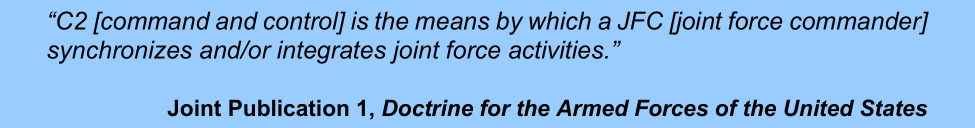
\includegraphics[width=0.7\paperwidth]{jptextex.png}

    \item Image tirée du \jp{}:

    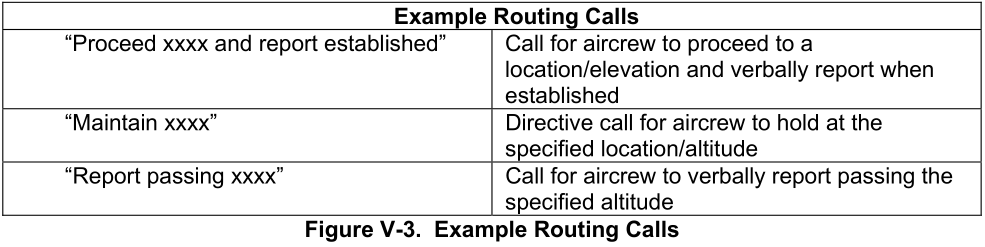
\includegraphics[width=0.7\paperwidth]{routing.png}

    \item Communication radio:
    \begin{lstlisting}
        Sochi sol, REDWOLF, pour la mise en route
        REWOLF, Sochi sol, QNH 0758, vent calme, mise en route approuv"é"e, rappelez pr"ê"t "à" rouler
    \end{lstlisting}

    \item \textbf{Emphase forte.}

    \item \emph{Emphase légère.}

    \item \important{Information importante.}
    
    %\item \useful{Information utile.}
    
    \item \remark{Remarque ou ensemble cohérent.}

    \item \note{Contenu, suggestion ou opinion qui n'est pas extrait du \jp{}.}

\ed 
%\import{./intro/}{conventions.tex}

\nocite{*}
\printbibliography[heading=bibintoc, title=Bibliographie]

\newpage

\pagenumbering{arabic}

\renewcommand{\cftdot}{.}

\tableofcontents

\addtocontents{toc}{\protect{\pdfbookmark[0]{\contentsname}{toc}}}

\newpage

\pagestyle{default}

\chapter{Introduction}

\begin{center}
    \makebox[\textwidth]{
\includegraphics[width=\paperwidth]{quote1.png}}
\end{center}

\e
	
    \item 
	Bien que l'objectif principal du \gls{cas} soit de fournir un cadre de travail dans des conditions bien spécifiques, les techniques décrites dans ce manuel peuvent être appliquées à toute situation nécessitant un \gls{tac}.%
\ed

\section{Aperçu}

\e
    \item
    Le \gls{cas} est une action effectuée par des appareils à voilure fixe ou à voilure tournante contre des cibles ennemies \textbf{proches des forces amies} et nécessite une \textbf{coordination étroite} entre les missions de support aérien et le mouvement des troupes amies.
    \item
    Le \gls{cas} est planifié et exécuté pour appuyer les unités amies au sol. Le \gls{cas} est étroitement intégré au niveau du contrôle tactique des forces amies supportées. Alors que l'affectation des ressources aériennes disponibles se fait au niveau stratégique opérationnel, le processus de planification du \gls{cas} se fait au niveau stratégique local, pour fournir aux unités amies au contact de l'ennemi un appui-feu précis et rapide.
    \item
    Le \gls{cas} peut être effectué partout ou les forces amies se trouvent au contact de l'ennemi. Le mot ``rapproché'' (``Close'') n'implique pas une distance spécifique, mais plutôt un contexte. Parfois, le \gls{cas} peut être le meilleur moyen d'exploiter une opportunité tactique en défense ou en attaque. Le \gls{cas} fournit un appui-feu capable de détruire, perturber, interdire, empêcher, harceler, neutraliser ou retarder l'ennemi.
    \item
    Chaque organisation s'entraîne et emploie le \gls{cas} en tant que partie d'une coalition. Le \gls{jfc} est responsable d'intégrer ces organisations au \gls{conops} en fonctions de leurs capacités.
    \item
    Le \gls{tac} est l'autorité responsable de manœuvrer les appareils de soutien aérien et d'autoriser l'attaque finale. Un \gls{jtac} ou un \gls{faca} certifié sera reconnu comme capable et autorisé à effectuer le \gls{tac}.
    \item
    Il y a trois types de contrôle (type 1, 2 et 3):
    \ee
        \item
        Contrôle de type 1

        Le contrôle de type 1 est utilisé lorsque le \gls{jtac}/\gls{faca} a besoin de contrôler de chaque attaque individuellement ainsi que d'avoir en permanence en visuel l'appareil qui attaque ainsi que sa cible.
        \item
        Contrôle de type 2

        Le contrôle de type 2 est utilisé lorsque le \gls{jtac}/\gls{faca} a besoin de contrôler chaque attaque mais qu'il ne peut pas voir l'appareil au moment du largage ou qu'il ne peut pas voir la cible.
        \item
        Contrôle de type 3

        Le contrôle de type 3 est utilisé lorsque le \gls{jtac}/\gls{faca} a besoin de contrôler chaque engagement, avec ses restrictions, mais qu'on engagement peut être composé de plusieurs attaques.
    \end{enumerate}
    Pour plus d'informations, voyez le chapitre: \nameref{controltypes}.
    \item \gls{tgo}: le personnel effectuant les \glspl{tgo} n'ont pas l'autorité pour contrôler les appareils engagés en opération \gls{cas} ou pour autoriser le tir.
\ed
    
\section{Usage du CAS}

\e
	\item
	L'usage du \gls{cas} s'inscrit dans le \gls{conops} de par sa spécificité à pouvoir frapper des cibles inaccessibles aux troupes au sol.
	
	\item
	Le \gls{gc} garde l'autorité suprême quant à l'usage d'armement dans sa zone de contrôle.
	
	\item
	Utilité sur le champ de bataille: le \gls{cas} permet au \gls{gc} de frapper l'ennemi rapidement et de manière inattendue.
	
	\item Critères pour l'usage du \gls{cas}:
	
	\ee
		\item Mission et \gls{conops}.
		\item Disposition, force et composition de l'ennemi.
		\item Capacités et limitations des appareils engagés dans le \gls{cas}.
		\item Emplacement et équipement des \gls{jtac}.
		\item \glspl{roe}.
		\item \gls{spins}.
		\item Défenses anti-aériennes ennemies et capacités alliées à les contrer.
		\item Disposition des forces amies
		\item Allocation des sorties \gls{cas}.
		\item Emplacement des civils et estimation des dommages collatéraux potentiels.	
	\ed
	
	\item Les cibles du \gls{cas} sont sélectionnées par le \gls{jtac}, en fonction des intentions du \gls{gc}, du terrain, de la météo, de la mission, des défenses ennemies, de l'armement disponible, du temps de réponse, etc. D'autres considérations peuvent entrer en ligne de compte.
\ed
	
\section{Intégration du CAS}
\e
	\item Lors des opération conjointes, l'intégration du \gls{cas} commence au niveau opérationnel. S'il est établi, le \gls{jfacc} fournit ses recommandations au \gls{jfc}. Chaque composante informe le \gls{jfc} de ses besoins et limitations. Le \gls{jfc} implémente le cadre dans lequel les opérations d'interdiction (\gls{cas}, \gls{ai}, etc.) s'intégreront dans l'\gls{opord}, l'\gls{aod}, l'\gls{ato}, l'\gls{aco} et les \gls{spins}.
\ed

\section{Emploi des voilures fixes et des voilures tournantes en opérations de CAS}

\e
	\item
	La structure organisationnelle, la mission principale et les capacités des appareils capables d'effectuer le \gls{cas} déterminent leur emploi. Bien que les \glspl{fw} et les \glspl{rw} puissent tous deux effectuer le \gls{cas}, leur emploi diffère.
	
	\item
	De par leur vitesse et leur portée opérationnelle, les \glspl{fw} offrent une grande versatilité et une grande flexibilité. De plus, ils emploient un arsenal de munitions très varié, qui peut être employé par presque toutes les conditions (météo, luminosité, ...).
	
	\item
	Les \glspl{rw} permettent de manœuvrer et de repositionner rapidement la puissance de feu en fonction de l'évolution de la situation. Ils ont un excellent temps de réponse et peuvent rester longtemps sur zone, peuvent évoluer à très faible altitude, et peuvent effectuer du \gls{cas} sur tous les types de terrain. Ils offrent également des capacités d'infiltration et d'extraction du personnel.

\ed

\section{Efficacité du CAS}

\e
	\item 
	Pour que le \gls{cas} soit efficace, il faut:
	\ee
		\item Du personnel correctement entraîné \\
		L'entraînement au \gls{cas} doit intégrer toutes les manoeuvres et procédures nécessaires à l'exécution du \gls{cas}. Cet entraînement doit être tenu à jour.
		\item Un planning et une intégration réfléchie \\
		Un \gls{cas} efficace s'appuie sur une planification en profondeur. La capacité à fournir la puissance de feu nécessaire au bon endroit est possible de par l'intégration avec les forces au sol. De point de vue du planificateur, le \gls{cas} pré-planifié sera toujours préféré.
		\item Un \gls{cc} efficace \\
		Le \gls{cas} nécessite une structure \gls{cc} flexible et intégrée au reste du dispositif pour trier les demandes, assigner les priorités, assigner les tâches, repositionner les éléments, fournir les alertes de menaces, et augmenter les capacité de \gls{cid}.
		\item Une supériorité aérienne établie (tout particulièrement le \gls{sead})
		\item Une reconnaissance et une connaissance des cibles
		\item Des procédures flexibles et éprouvées
		\eee
			\item Placement des unités de \gls{cas} proche de leur zone d'opération. Placement des points d'attente de d'orbite de manière optimiser le temps de réaction.
			\item Délégation des autorisations de tir aux unités subordonnées.
			\item Ré-assignation des appareils en fonction des situations émergentes.
			\item Révision de l'\gls{ato} en fonction des situations émergents.
			\item Redirection des appareils \gls{cas} en réponse aux menaces.
			\item Délégation des autorité au plus bas niveau tactique possible.
			\item Placement des \gls{jtac} avec les unités au sol de manière à faciliter les communications et la coordination avec les appareils de \gls{cas}.			
		\ed
		\item De l'armement approprié \\
		Le \gls{gc} et le \gls{jtac} doivent connaître l'effet de l'armement employé, de manière à pouvoir évaluer les possibilités de dommages collatéraux, et l'impact sur le poursuite de la mission.
		\item Des conditions environnementales \\
		Des conditions favorables améliorent l'efficacité des unités de \gls{cas} quelles que soient les capacités de l'appareil ou de l'armement. \textbf{Avant d'envisager une mission de \gls{cas}, des conditions météo minimales doivent être définies}. Certaines conditions peuvent n'influencer que certaines plateformes; par exemple, un plafond très bas peut rendre certains \glspl{fw} inutiles, sans impacter les \glspl{rw}. Inversement, les \glspl{fw} pourront opérer lors d'une tempête de sable qui clouerait les \glspl{rw} au sol. Les conditions météo influencent également fortement le marquage de la cible.	
		
	\ed
\ed

\section{Responsabilités}

\e
	\item \gls{jfc} \\
	Le \gls{jfc} établit le cadre et les priorités pour le \gls{cas} dans le \gls{conops}.
	
	\item \gls{jfacc} \\
	Le \gls{jfacc} reçoit du \gls{jfc} l'autorité pour créer des missions et des tâches.
	
	\item \note{Le commandant d'escadron s'assure que ses unités sont capables d'exécuter des missions de \gls{cas}}
\ed
	
\section{Minimiser le tir fratricide}

\e
	\item Le tir fratricide est parfois le résultat tragique de la guerre.
	\item
	\textbf{Bien que parfois le résultat d'armement défectueux, le tir fratricide est souvent le résultat de la confusion qui règne sur le champ de bataille.}
	\note {Kakane, celle-là est pour toi !}
	Les causes peuvent être, entre autres:
	\ee
		\item Mauvaise identification de la cible
		\item Position ou description de la cible erronée
		\item Mauvaise transmission de la position ou de la description de la cible
		\item Perte de \gls{sa} par le pilote ou le \gls{jtac}
	\ed
	\item Responsabilités \\
	Tout le personnel impliqué dans le \gls{cas} est responsable de la sécurité lors du planning et de l'exécution. Chaque participant doit tout entreprendre pour identifier les unités alliées, les forces ennemies et les civils avant de prendre pour cible, d'engager, ou d'autoriser le tir.
	\item Entraînement \\
	La coalition, ses composantes, et les unités doivent effectuer un entraînement conjoint régulier qui simule des opérations réelles de manière à développer les capacités nécessaires au bon déroulement du \gls{cas}.	
\ed

\section{Minimiser les victimes civiles}
\e
	\item Les lois de la guerre obligent tous les commandants à prendre toutes les précautions nécessaires pour minimiser les victimes civiles et les dégâts collatéraux.
\ed


\chapter{Command and Control}

\begin{center}
    \makebox[\textwidth]{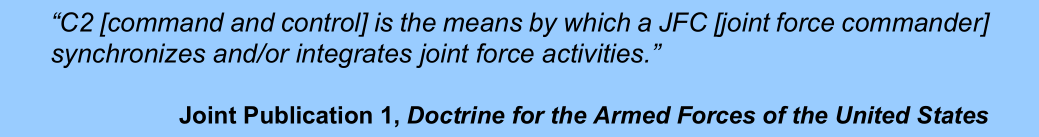
\includegraphics[width=\paperwidth]{quote3.png}}
\end{center}

\chapter{Planification et demande}

\e
    \item Il existe deux types de \gls{cas} distincts:
    \ee
        \item Le \gls{cas} planifié
        \item Le \gls{cas} immédiat
    \ed
\ed

\section{Le CAS planifié}

\e
    \item Le ``\gls{cas} request'' est effectué par l'unité qui demande un soutien aérien. On distingue deux principaux types de demandes:
    \ee
        \item Le \gls{cas} planifié à l'avance (``pre-planned \gls{cas}'', ou simplement ``\gls{cas}'')
        \item Le \gls{cas} ``à la demande'' (``on-call cas''), qui regroupe deux possiblités:
        \eee
            \item Le \gls{xcas}, où l'appareil en attente de tasking se trouve déjà dans les airs
            \item Le \gls{gcas}, où l'appareil en attente de tasking se trouve encore au sol
        \ed
    \ed
    \item Un ``\gls{cas} request'' réel se compose d'un grand nombre d'informations, utiles à la planification de la mission et à la répartition des effectifs disponibles.
    \item
    Souvent, pour DCS, l'équivalent du ``\gls{cas} request'' sera contenu dans le briefing de la mission (zone d'opération, menace, composition et force de unités ennemies, timing, emport, unités amies, \gls{jtac}, plan de fréquences, etc…).
    \item Toute référence ultérieure au ``\gls{cas} request'' fera donc implicitement référence au briefing de mission.
    \item Les considération à prendre en compte lors de l'établissement d'une \gls{cas} request sont propres au rôle de \gls{gc}/\gls{jfc} et ne seront pas traitées dans ce document.
    \item Le \gls{cas} planifié est un \gls{cas} effectué après une requête spécifique, concernant une zone connue, pour atteindre un objectif déterminé.
    \item Dans le cas d'un \gls{cas} planifié, un grand nombre de paramètres sont connus avant le décollage, ce qui permet une meilleure préparation.
\ed

\subsection{Étape 1: réception de l'ordre de mission}

\e
    \item
    En tant que participants au processus de planification, les officiers en charge (chef de patrouille, commandant d'escadron, …) devraient être à même de comprendre et analyser l'information à partir de ces différentes sources:
    \ee
        \item \gls{aob}
        \item \gls{ato}
        \item \gls{aco}
        \item \gls{spins}
        \item \gls{opord}
        \item \gls{sop}
    \ed
\ed
\note{Les \glspl{sop} sont propres à l'escadron, et sont normalement connues par les tous les officiers supérieurs.
    
    Exceptés les \glspl{sop}, tous les éléments sont normalement fournis sous une forme ou l'autre dans le briefing de mission.
    
    S'il devait manquer un élément, il appartient à l'officier en charge de la patrouille d'évaluer son importance et de poser les questions nécessaires à l'organisateur de la mission.
}

\subsection{Étape 2: analyse de la mission} 

\e
    \item Avant de pouvoir préparer la mission, les officiers en charges devront:
    \ee
        \item Mettre à jour les différentes sources d'informations (\gls{ato}, \gls{spins}, \gls{aco}, …)
        \item Estimer les capacités des forces à leur disposition (équipement, personnel, restrictions, …)
        \item Déterminer les tâches essentielles de la mission
        \item Évaluer les conditions relatives à:
        \eee
            \item L'ennemi
            \item La météo
            \item Le terrain
        \ed
        \item Avertir les unités (personnes) subordonnées
    \ed
    \item Considérations clefs à prendre en compte lors de l'analyse de la mission:
    \ee
        \item \gls{conops}: Quelles sont les intentions du \gls{jfc}? Attaque ou de défense? Surprise ou délibéré? Règles d'engagement?
        \item Comment s'intègre le \gls{cas} au reste du dispositif?
        \item Quelles pourraient être les intentions de l'ennemi? Comment ces intentions sont-elles affectées par le terrain, la météo, l'heure ?
        \item Quels sont les moyens de surveillance ou de reconnaissance à notre disposition?
        \item \gls{complan} Comment vont s'organiser les communications? Est-ce que toutes les unités participantes au \gls{cas} sont intégrées au \gls{complan}  de manière fiable et redondante?
    \ed
    \item Dans le cas d'une demande de \gls{cas} pré-planifié, un grand nombre d'informations supplémentaires pourront être obtenues via la demande elle-même. Par exemple:
    \ee
        \item Zone de \gls{cas}
        \item Menaces
        \item Type de cibles
        \item Localisation de la cible
        \item Localisation des forces amies
        \item Type de terrain
        \item Restrictions horaires
        \item \gls{jtac}
    \ed
\ed

\subsection{Étape 3: préparation de la mission}

\begin{center}
    \makebox[\textwidth]{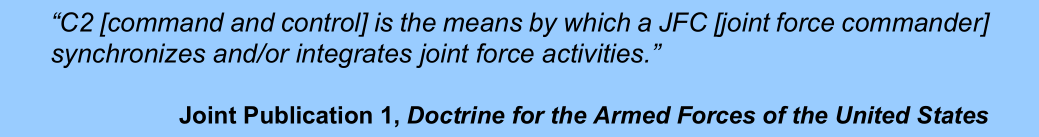
\includegraphics[width=\paperwidth]{quote2.png}}
\end{center}

\e
    \item Le ``Mission planning'', ou ``préparation de la mission'', est une étape cruciale au bon déroulement de cette dernière.
    \item Cette préparation sera effectuée par le chef de patrouille, qui sera chargé de rassembler et analyser toutes les informations à sa disposition pour préparer au mieux la mission de la patrouille dont il a la charge.
    \item Lorsque c'est possible, la préparation de la mission se fait en collaboration avec les différents éléments impliqués, certainement avec le \gls{jtac} en charge de la zone attribuée à la patrouille, le \gls{tacon}, et les autres chefs de patrouilles opérant dans le même théâtre opérationnel.
    \item Le chef de patrouille veillera tout particulièrement à toujours utiliser les informations les plus récentes, et fera attention à se tenir au courant de l'évolution de la situation.
    \item Il devra également s'assurer que tous les éléments sous son contrôle ont reçu et compris ses intentions pour la mission.
    \item Checklist de préparation de mission: \fullref{ann1}
\ed

\section{Le CAS immédiat}

\e
    \item Le \gls{cas} immédiat intervient lorsque la situation sur le champ de bataille évolue de manière inattendue.
    \item L'\gls{ato} peut allouer un certain effectif pour se préparer à répondre à ces situations.
    \item Le chef de patrouille trouvera alors dans cet \gls{ato} les informations nécessaires pour préparer son vol (emport, point d'attente, etc…).
    \item
    Pendant le vol (ou au parking pour le \gls{gcas}), si l'intervention de la patrouille s'avère nécessaire, celle-ci recevra un point de contact initial, ainsi que le call-sign et la fréquence de l'agence qui s'occupera de son contrôle terminal.
\ed







\chapter{Préparation}

\chapter{Exécution}

\begin{center}
    \makebox[\textwidth]{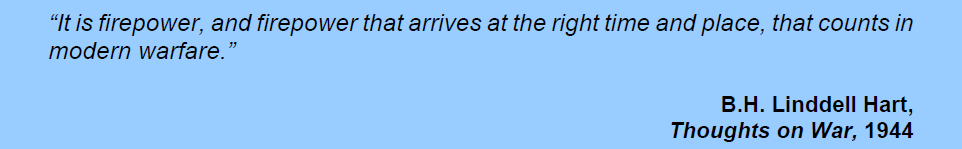
\includegraphics[width=\paperwidth]{quote5.png}}
\end{center}

\section{Introduction}

L'exécution du \gls{cas} commence lorsque la cible est désignée par le \gls{gc} soutenu, et décrit les considérations à prendre en compte pour intégrer le \gls{cas} aux manoeuvres de l'unité soutenue.

\section{Engagement de la cible lors du CAS}

Cette section décrit les procédures standard lors du \gls{cas}. Bien que certaines opérations nécessitent des procédures spécifiques, le personnel impliqué dans le \gls{cas} doit être familier avec le format standard.

\subsection{Création du briefing par le J-TAC}
Cette sous-section décrit les tâches que doit effectuer le \gls{jtac} une fois que la cible a été désignée par le \gls{gc}.

\e
    \item Rassembler les informations à propos de la cible
    \ee
        \itemt{Élévation de la cible (ligne 4)}{
        Par défaut, l'élévation est exprimée en pieds au dessus de la mer (ft \gls{msl})}
        \itemt{Description de la cible (ligne 5)}{
        La description de la cible doit être concise et précise (par ex. ``5 chars dans un champ''). Le \gls{jtac}/\gls{faca} doit éviter d'utiliser des descriptions compliquées ou des termes qui risquent de ne pas être compris par les pilotes. Cependant, la descrition doit rester spécifique. si le \gls{gc} veut attaquer une \gls{hvt} qui se trouve dans un building à deux étages, il devra spécifier "\gls{hvt} dans building à 2 étages", et pas seulement "building à 2 étages".}
        \itemt{Position de la cible (ligne 6)}{
        Le \gls{jtac}/\gls{faca} doit évaluer la précision minimale nécéssaire pour les coordonnées de la cible pour accomplir les objectifs du \gls{gc}. Un largage de bombe guidée laser depuis un émetteur au sol demandera des coordonnées beaucoup moins précises qu'une largage de \gls{jdam}.}
        \eee
            \itemt{Association du terrain et d'une carte}{
            Le moins précis, mais rapide et efficace en fonction de la situation.}
            \itemt{\gls{lrf} couplé au \gls{gps} et/ou la boussole}{
            Sujet à l'imprécision de la boussole, et au brouillage \gls{gps}. Si le brouillage \gls{gps} est possible, une autre méthode devra être utilisée.}
            \item Logiciel de ciblage
            \item Coordonnées dérivées des images de reconnaissance
        \ed
        \itemt{Positions alliées (ligne 8)}{
        La positions des unités alliées au sol sont données à partir de la position de la cible. La direction est donnée de manière cardinale ou sous-cardinale, et la distance est exprimée en mètres. L'observateur ou le \gls{jtac} peuvent ne pas être l'unité alliée la plus proche de la cible.}
        \itemt{Effet souhaité par le \gls{gc}}{
        L'effet souhaité par le \gls{gc} est déterminé en parlant avec lui. Le \gls{jtac} doit offrir au \gls{gc} une estimation réaliste des possibilités en fonction des appareils disponibles, de l'armement embarqué, et de son expertise.}
    \ed
\ed
\subsection{Requête de CAS}
\e
    \item Une fois que la position de la cible a été grossièrement estimée, le \gls{jtac} doit envoyer la demande de \gls{cas} le plus vite possible, pour prendre en compte le temps nécessaire avant l'arrivée des appareils. Il ne faut pas retarder l'envoi de la demande pour augmenter la précision des coordonnées de la cible.\\ \important{Il ne faut jamais utiliser les coordonnées des unités alliées comme coordonnées cible dans une demande de \gls{cas}.}
    \itemt{Création du game plan}{
    Au minimum, le game plan contiendra le type de contrôle et la méthode d'attaque. D'autres informations peuvent être intégrée au game plan ou être ajouté plus tard aux remarques du CAS brief: les intentions du \gls{gc}, l'effet désiré, l'intervalle entre les appareils dans le cas d'une attaque simultanée par plusieurs éléments \gls{cas}. Dans le cas d'attaques séquentielles (\gls{sead}, marquage), une attention particulière devra être apportée à l'établissement de la séparation entre les appareils. L'objectif du \gls{jtac} n'est pas de dicter aux appareils de \gls{cas} les tactiques à employer, mais de fournir un plan qui correspond aux intentions du \gls{gc}.}
    \ee
        \itemt{Déterminer l'effet désiré}{
        \remark{
        \eee
            \item Composition de la cible (blindage)
            \item Répartition de la cible (centré sur un point ou dispersé)
            \item Position (dégagée ou protégée)
            \item Dégâts collatéraux potentiels
            \item Proximité des unités alliées
        \ed}}
        \itemt{Choisir le type de \gls{tac}}{
        Le type de \gls{tac} dépend de l'armement employé, de la manière manière de réduire les risques, de la vitesse de l'engagement et de la capacité du \gls{jtac} à voir la cible et/ou l'appareil qui attaque.}
        \itemt{Choisir la méthode d'attaque (\gls{boc} ou \gls{bot})}{
            La méthode d'attaque est choisie de manière à permettre l'attaque la plus rapide possible, en fonction du type de cible, de la façon dont sera acquise la cible, et de la situation}
        \itemt{Planifier l'intervalle entre les appareils}{
        Le \gls{jtac} peut demander un intervalle spécifique entre les attaques, en fonction de la cible, des menaces, des activités alliées, de la déconfliction artillerie/\gls{sead}/laser, de l'armement utilisé, des restrictions, de la météo, etc. Les pilotes se doivent d'adapter leur tactiques pour respecter le timing et les intervalles imposés.}
        \eee
        	\itemt{Attaque simultanée}{
        	Tous les appareils délivreront leur armement de manière à créer un effet simultané. Cette méthode minimise l'exposition des appareils aux menaces et offre à l'ennemi un temps de réaction très court. C'est la méthode optimale pour engager des cibles multiples, tout particulièrement des cibles mobiles qui pourraient fuir après la première attaque. Le principal désavantage de cette méthode est l'impossibilité de corriger ou d'annuler le tir entre les impacts et la diminution du support mutuel entre les appareils qui attaquent.\\
        	\important{Un attaque simultanée nécessite que les appareils utilisent des codes laser différents.}}
        	\itemt{Attaque séquentielle}{
        	Les appareils attaquent un à la fois, avec un intervalle spécifique entre les attaques, basé sur le temps nécessaire à l'acquisition de l'appareil précédent, la durée de vol de l'arme employée, le temps nécessaire au dégagement visuel de la zone attaquée (fumée, fragments, etc.), et le temps nécessaire à évaluer l'efficacité de la frappe précédente et le besoin d'une nouvelle frappe.\\ Quelques guides pour les attaques séquentielles:
        	\eeee
        		\item 30 secondes pour un contrôle de type 1 avec des bombes lisses
        		\item 1 minute pour des \gls{lgb} délivrées à altitude moyenne
        		\item Plus de deux minutes pour décider de la ré-attaque lors de l'emploi de \gls{pgm} à haute ou moyenne altitude
        	\ed}
        \ed
    \ed
    \item Détermination du type de marque et de l'aide à la corrélation
    \ee
    	\itemt{\gls{boc}}{
    	\eee
    		\item Pas de marque nécessaire (ligne 7: "No mark")
    		\item Si le \gls{tac} est utilisé avec des \gls{lgw}, le call-sign de l'unité qui fournit le \gls{tac} et le code laser seront fournis.\\ (ligne 7 (exemple): "Blackjack laser, code 1688")
    	\ed}
    	\itemt{\gls{bot}}{
    	La marque dépendra de l'appareil qui attaque}
    	\item \gls{bot} et contribution d'une tierce partie
    	\eee
    		\itemt{Tierce partie}{
Suite l'expansion des technologies déployées sur le champ de bataille, le \gls{jtac} peut décider de recourir à une tierce partie (unité \gls{recce}, sniper, appareils équipés d'un émetteur laser, etc.) pour aider à l'obtention des coordonnées ou de la position de la cible, à l'attaque terminale ou à l'établissement du \gls{bda}. De ce fait, la corrélation avec ces parties tierces sera également nécessaire.}
\item Considérations
			\eeee
				\item Les pilotes utilisent généralement une combinaison de senseurs et leurs yeux pour acquérir les marques et les cibles. Le \gls{jtac} doivent être familiers avec les capacités des senseurs et utiliser des marques qui utilisent ces capacités.
				\item Le \gls{jtac} doit toujours avoir en réserve un plan de marquage alternatif.
			\ed
			\item Types de marque et \gls{tgo}
			\eeee
				\itemt{Marquage laser}{
				Le passage de la marque laser est le fait d'utiliser un \gls{ltd} pour fournir l'énergie laser au \gls{lst} de l'appareil. Le \gls{ltd} peut se trouver au sol ou embarqué dans un autre appareil.}
				\eeeee
					\item Avantages
					\eeeeee
						\item Excellente corrélation de la position de la cible si la géométrie correcte est utilisée
						\item Peut être utilisé de jour comme de nuit
					\ed
					\item Désavantages
					\eeeeee
							\item Nécessite un \gls{ltd} et un \gls{lst}
							\item Demande de la coordination géométrique pour le \gls{lst} ne traque pas le \gls{ltd} (l'origine du pointage)
							\item Le marquage laser depuis le sol est souvent difficile, particulièrement lorsque l'unité qui effectue le pointage est sous le feu ennemi
							\item Un premier passage d'acquisition de la marque est parfois nécessaire
					\ed
				\important{Lors du marquage laser depuis le sol, un \gls{fah} sera obligatoirement donné, de manière à renforcer l'établissement de la géométrie correcte}
				\ed
				\itemt{Marquage infrarouge (\acrshort{sparkle})}{
				Les pilotes utiliseront leur \gls{nvg} pour acquérir la cible.\\
				\important{Les pilotes doivent appeler "VISUEL SPARKLE", "TALLY SPARKLE" ou "CONTACT SPARKLE" quand un marquage infrarouge est utilisé à partir du sol}
				\eeeee
					\item Avantages
					\eeeeee
						\item Rapide
						\item Le \gls{jtac} a la confirmation visuelle que le pilote a bien acquis la cible correcte							
					\ed
					\item Désavantages
					\eeeeee
						\item De nuit seulement
						\item Requiert de la coordination géométrique pour s'assurer que le pilote a bien acquis la fin du faisceau infrarouge et non pas sa source
						\item S'il y a plusieurs pointeurs \gls{ir} près d'une même cible, il devient difficile pour le \gls{jtac} de déterminer si le pointeur se trouve bien sur la cible à cause du phénomène de ``diffusion'' dans les \gls{nvg}
						\item Si l'ennemi dispose également de \gls{nvg}, l'utilisation d'\gls{ir} expose l'opérateur et supprime le facteur de surprise
					\ed
				\ed}
				\itemt{Marquage à partir d'un \gls{trp}}{
				\eeeee
					\item Avantages
					\eeeeee
						\item Prêt rapidement si le pilote connaît le \gls{trp}
						\item De jour comme de nuit
						\item Offre un point de référence commun pour le talk-on
					\ed
					\item Désavantages
					\eeeeee
						\item Nécessite le pilote connaisse le \gls{trp}
					\ed
				\ed}
				\itemt{Marquage \gls{idf} (fumigène)}{
				\eeeee
					\item Avantages
					\eeeeee
						\item De jour comme de nuit (obus phosphorescents ou lumineux)
						\item Le \gls{jtac} ne doit pas dévoiler sa position
						\item Offre un point de référence commun pour le talk-on
					\ed
					\item Désavantages
					\eeeeee
						\item Prend du temps à coordonner
						\item Le manque de précision implique souvent une correction supplémentaire à partir de la marque
						\item Le tire indirect implique une déconfliction supplémentaire
						\item Le \gls{fov} des senseurs peut être un problème si la marque se trouve en dehors
						\item L'illumination de nuit sature les \gls{nvg}
						\item Sacrifie l'effet de surprise
					\ed
				\ed}
				\itemt{Marquage par feu direct}{
				Utilise un tir direct (munitions traçantes ou grandes fumigènes) pour marquer la cible
				\eeeee
					\item Avantages
					\eeeeee
						\item Facilement accessible
					\ed
					\item Désavantages
					\eeeeee
						\item Risque de dommages collatéraux
						\item Difficulté pour les \gls{rw} d'acquérir visuellement la marque de jour
						\item Difficulté pour les \gls{fw} d'acquérir visuellement la marque de jour comme de nuit
						\item Le \gls{fov} des senseurs peut être un problème si la marque se trouve en dehors
						\item L'illumination de nuit sature les \glspl{nvg}
						\item Sacrifie l'effet de surprise
					\ed
				\ed}
				\itemt{Considérations pour le marquage de nuit}{
				\eeeee
					\item La visibilité limitée et le manque de perspective rend la corrélation de nuit difficile
					\item L'illumination du champ de bataille doit être planifiée de manière à ne pas saturer les \glspl{nvg}
				\ed}
				\itemt{Marques d'opportunité}{
				N'importe quoi sur le champ de bataille peut servir de marque; un bâtiment en feu, le trafic routier, etc.}
			\ed
       	\ed
    \ed
    \item Détermination la géométrie d'attaque reprise 227 TODO
\ed


\e
    \item Déroulement d'une mission \gls{cas}:
    \begin{figure}[H]
        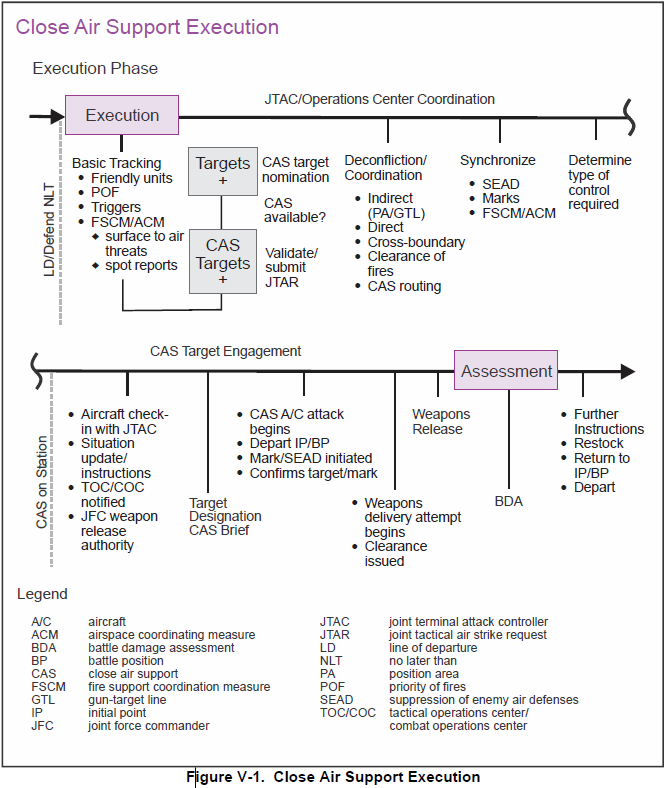
\includegraphics[width=\textwidth]{execution-full.png}
        \caption{Déroulement d'une mission.}
        \label{fig:casflow-full}
    \end{figure}
    \item Cas flow simplifié:
    \begin{figure}[H]
        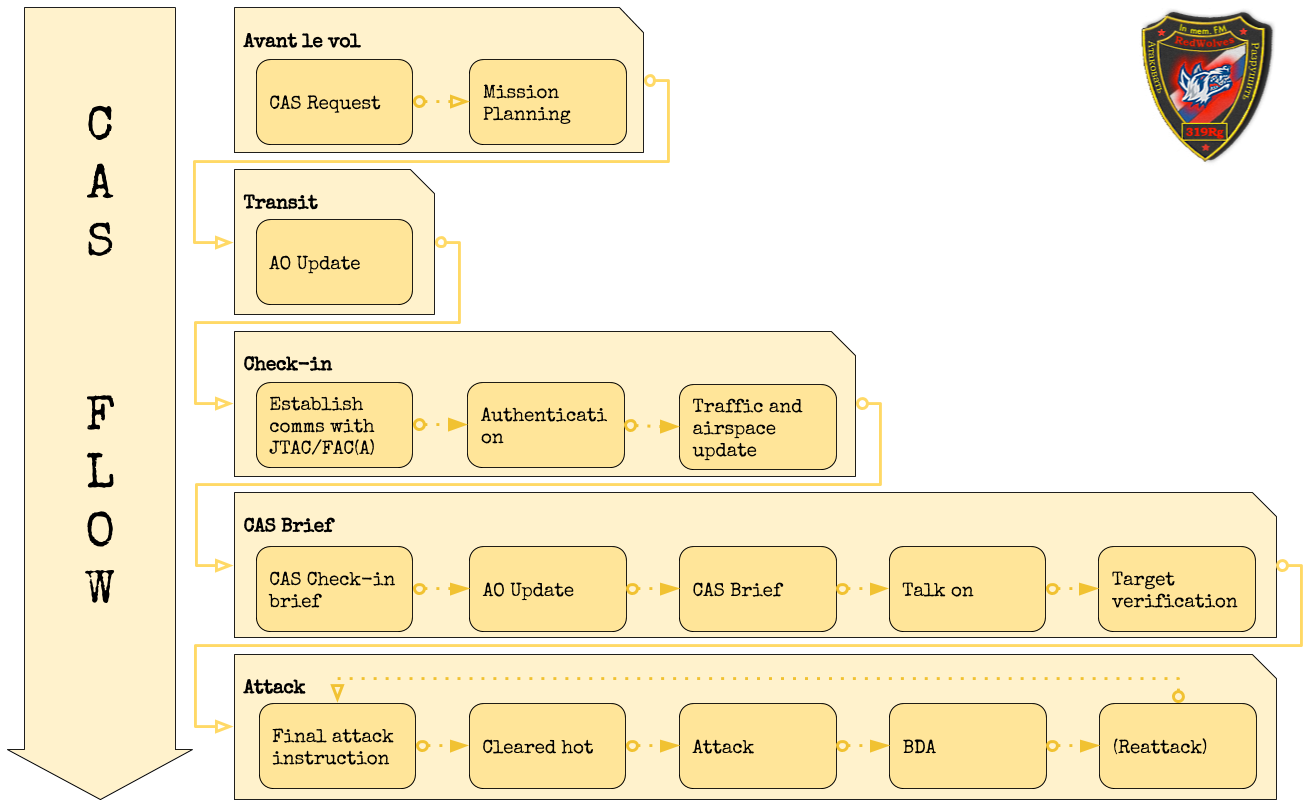
\includegraphics[width=\textwidth]{CASFlow.png}
        \caption{Cas flow simplifié.}
        \label{fig:casflow}
    \end{figure}
\ed

\e
    \item
    Ce chapitre présente le déroulement pratique d’une mission \acrshort{cas}. Le template qui y est présenté illustre une mission \acrshort{cas} typique, et fournit un guide pour le \acrshort{jtac}/\acrshort{faca} et le pilote pour les aider à remplir leur mission.
    \item Le déroulement présenté ici commence après le décollage, et se termine lorsque la patrouille de \acrshort{cas} est sur le retour.
\ed

\section{Routing}
\e
    \item Le routing consiste à diriger les appareils d’un point à un autre.
    \item Extrait du \jp:\\
    \begin{figure}[H]
        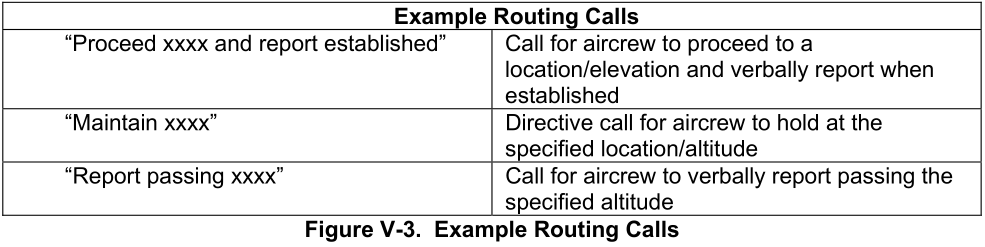
\includegraphics[width=\textwidth]{routing.png}
        \caption{Routing.}
        \label{fig:routing}
    \end{figure}
    \item Exemples:\\
    \ee
        \item Routing standard, demande de maintien de position:\\
        \begin{figure}[H]
            
\includegraphics[width=\textwidth]{routing_ex1.png}
            \caption{Routing: maintien de position.}
            \label{fig:routingpos}
        \end{figure}
        \item Si le contrôleur n'est pas certain de la position et de l'altitude de l'appareil, il doit demander les informations:\\
        \begin{figure}[H]
            
\includegraphics[width=\textwidth]{routing_ex2.png}
            \caption{Routing: demande d'information.}
            \label{fig:routinginfo}
        \end{figure}
        \item Ordre de se diriger vers un point:\\
        \begin{figure}[H]
            
\includegraphics[width=\textwidth]{routing_ex3.png}
            \caption{Routing: ordre.}
            \label{fig:routingorder}
        \end{figure}
        \item Information relative à une menace:\\
        \begin{figure}[H]
            
\includegraphics[width=\textwidth]{routing_ex4.png}
            \caption{Routing: information menace.}
            \label{fig:routingthreat}
        \end{figure}
        \item Information relative aux activités alliées:\\
        \begin{figure}[H]
            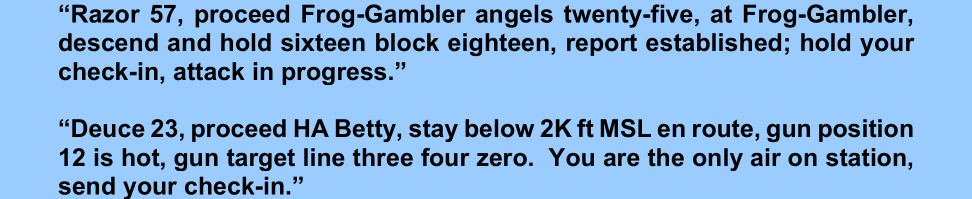
\includegraphics[width=\textwidth]{routing_ex5.png}
            \caption{Routing: information alliés.}
            \label{fig:routingallies}
        \end{figure}
    \ed
\ed

\section{Check-in}

\e
	\begin{minipage}{\linewidth}
    \item
    Le check-in est la première phase du \acrshort{cas} en tant que tel. C’est l’appel effectué de l’appareil en \acrshort{cas} vers le \acrshort{jtac}/\acrshort{faca} pour lui signifier qu’il est prêt à remplir sa mission de \acrshort{cas}.
    \item Comme le check-in peut prendre un certain temps, un appel préliminaire devrait être effectué. Par exemple:
	\begin{lstlisting}[caption=Appel préliminaire, label=preliminary_call]
    PIRATE, ici REDWOLF, pour check-in, quand dispo.
	\end{lstlisting}
	\end{minipage}

	\begin{minipage}{\linewidth}
    \item Format du check-in:
    \begin{figure}[H]
        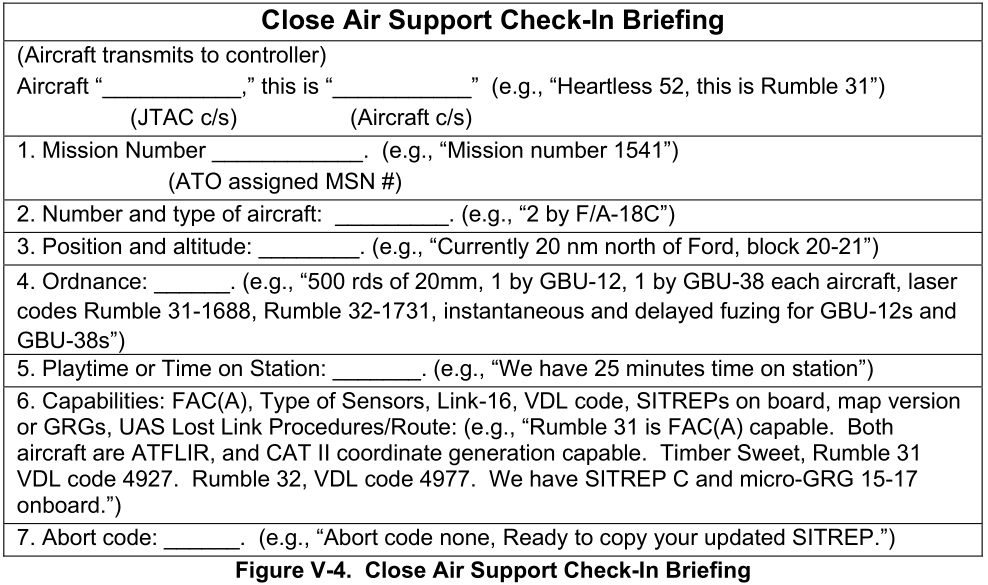
\includegraphics[width=\textwidth]{checkin.png}
        \caption{Format check-in.}
        \label{fig:checkin}
    \end{figure}    
    \end{minipage}
    
    \begin{minipage}{\linewidth}
    \item S'il le souhaite, le \gls{jtac}/\gls{faca} peut demander un check-in abrégé:
    \begin{figure}[H]
        
\includegraphics[width=\textwidth]{abbregcheckin.png}
        \caption{Format check-in abrégé.}
        \label{fig:abbregcheckin}
    \end{figure}
    \end{minipage}
    
    \item Le code d’annulation (ligne 7) est un code alphabétique servant à authentifier la directive “Abort” du J-TAC/FAC(A).
    
    \begin{minipage}{\linewidth}
    \item Exemple de check-in:
    \begin{lstlisting}[caption=Check-in, label=checkin]
	PIRATE ici REDWOLF
    	Mission 1234
	    2 Kamov
	    20km au sud de Poti, 500m MSL
    	24 Vikhrs, 80 roquettes, full guns
	    Playtime 30 minutes
    	Senseurs: Shkval
	    Abort code: X-RAY TANGO ZULU
	\end{lstlisting}
    \end{minipage}
\ed


\chapter{Communications}

\e
    \item Les participants au CAS utiliseront les réseaux radios des unités qui requièrent le soutien aérien.
    \item
    De façon plus spécifique, les unités capables d’effectuer le CAS auront besoin des fréquences radios et des call-signs utilisés par les différentes agences, unités au sol, et J-TAC qu’elles seront susceptibles d’avoir à contacter.
    \item Voici une simplification des différents réseaux radios utilisés lors du CAS (tous ``voice''):
    \ee
        \item Army Command/Operation Net: réseau utilisé par les GCs.
        \item Fire Support Net: réseau utilisé pour les demandes d’appui-feu.
        \item Air Control Net: réseau utilisé par les différentes agences et unités de contrôle pour coordonner les différentes unités sous leur contrôle.
        \item C2Net: interface entre les différentes unités et agences de contrôle.
        \item Guard Net: fréquence de garde; lorsque c’est possible, toute unité engagée en opération sera à l’écoute de ce réseau.
        \item INFLTREP: utilisé pour le MISREP pendant l’egress
    \ed
\ed


\chapter{Tactiques de CAS RWs}

\e
    \item Ce chapitre aborde certaines des tactiques particulières au \gls{rw}. Ces tactiques évoluent en permanence et doivent être adaptées en fonction de la situation.
    \item \important{La décision finale d’utiliser telle ou telle tactique revient toujours au chef de patrouille, mais ce dernier doit veiller à se plier aux contraintes imposées par le \gls{jtac}/\gls{faca}.}
\ed

\section{Altitude d’opération}

\e
    \item Pour une patrouille \acrshort{rw}, on définit l’altitude comme suit:
    %\ee
    	\remark{%
    	\ee
        \item Haut: au dessus de 1000m sol
        \item Moyen: entre 200m et 1000m sol
        \item Bas: en dessous de 200m sol
        \ed
        }%
    %\ed
\ed

\section{Lancement et récupération}

\e
    \item
    Les unités \gls{rw} peuvent opérer à partir de base aérienne ou de points avancés (uniquement les \glspl{farp} dans DCS), ce qui les place au plus près de la ligne de front et prêts à intervenir rapidement.
\ed

\section{Communication durant le transit}

\e
    \item
    Du fait de leur capacité à évoluer à faible altitude, il est souvent difficile pour le \gls{cc} de maintenir une communication constante avec les unités \gls{rw}.
    \item
    Cette difficulté est à prendre en compte lors de la préparation de la mission,  et un système alternatif doit être mis en place pour assurer les communications entre les unités \gls{rw} et leur \gls{tacon}.
\ed

\section{Tactiques durant le transit}

\subsection{Objectifs}

\e
    \item Handicapées par leur faible vitesse, les unités \gls{rw} doivent mettre à profit leur manœuvrabilité pour:
    \ee
        \item Éviter les concentrations de défenses anti-aériennes ennemies
        \item Empêcher la détection le plus longtemps possible
        \item Rester en dehors de la portée de certains systèmes d’armes sol-air
    \ed
\ed

\subsection{Navigation}

\e
    \item Le profil de pénétration (route, altitude, vitesse, formation, suivi du terrain) doit être prévu de manière à atteindre ces objectifs.
    \item En plus des considération purement tactiques, d’autres facteurs entrent en ligne de compte:
    \ee
        \item La météo
        \item Le carburant
        \item Les défenses anti-aériennes alliées
    \ed
    \item Les profils de pénétration possibles sont regroupés en trois catégories:
    \remark{%
    \ee%
        \item Bas niveau: L’approche bas niveau se fait à vitesse et altitude constante (30-60m du sol).%
        \item Contour: Le vol de contour se fait en utilisant le terrain, les obstacles et la végétation pour occulter la formation à l’ennemi, généralement entre 15 et 30 mètres du sol.%
        \item \gls{noe}: Le vol \gls{noe} se fait aussi proche que possible du sol, à des vitesses et altitudes variables, qui dépendent du terrain, de la météo, de la luminosité et de l’ennemi
    \ed%
    }%
\ed

\subsubsection{Menaces particulières}

\e
    \item De par leur très faible altitude de navigation, les \gls{rw} sont vulnérables au tir d’armes de petit calibre et aux \glspl{rpg}.
    \item Certains situations nécessiteront que la patrouille évolue à altitude plus élevée.
    \item Pour ces mêmes raisons, une patrouille \gls{rw} évitera de survoler un environnement urbain (hors phase d’attaque).
\ed

\subsubsection{Jour et nuit}

\e
    \item L’altitude et la vitesse devront être adaptées en fonction de la luminosité ambiante en corrélation avec le type de terrain survolé.
\ed

\section{Tactiques de pénétration}

\e
    \item Les tactiques de pénétration sont d’application depuis l’arrivée en zone d’attente jusqu’au début de la phase d’attaque.
    \item En plus des positions de contrôles normales du CAS, les hélicoptères peuvent utiliser des positions spéciales: les \gls{ha} et les \glspl{bp}.
    \item Ces positions sont facultatives, et sont choisies par le chef de patrouille, en collaboration avec le \gls{jtac}, pour leur valeur tactique ajoutée.
\ed

\subsection{Points de référence spécifiques aux RWs}

\subsubsection{Holding Areas}

\e
    \item Les \glspl{ha} sont établies pour fournir aux \glspl{rw} une position d’attente sécurisée.
    \item Ces positions servent à “stacker” les \glspl{rw} entre deux tâches, à effectuer le \gls{cas} brief, ou quelqu’autre tâche nécessitant la pleine attention du pilote.
    \item Elles sont établies le plus près possible de la zone de combat, sans pour autant exposer les \glspl{rw} au feu ou à la détection.
\ed

\subsubsection{Battle Positions}

\e
    \item Les \glspl{bp} sont des zones de manoeuvres contenant des points des tir, permettant au \glspl{rw} de rester en constante évolution durant l’engagement.
    \item Elles sont établies de manière à faciliter l’ingress et l’egress, et à offrir une protection maximale aux \glspl{rw} en cas de riposte ennemie.
    \item Ces positions sont définies à l’avance ou lors du \gls{cas} brief.
\ed

\subsubsection{Firing Points}

\e
    \item Les \glspl{fp} sont des points situés dans une \glspl{bp}.
    \item La position exacte de ces points à la discrétion du pilote.
    \item Ces points sont établis de manière à:
    \ee
        \item Offrir au pilote une position de tir la plus sécurisée possible
        \item Permettre un repli rapide vers une position protégée en cas d'engagement par l'ennemi.
        \item Empêcher les conflit verticaux ou horizontaux entre les membres de la patrouille.
        \item Permettre l'engagement immédiat des cibles, ou dans un délai très court.
    \ed
\ed

\begin{figure}[H]
    \begin{minipage}{\textwidth}
        \subsubsection{Résumé des positions spécifiques aux \gls{rw}s}
        \e
            \item Extrait du \jp:\\
        \ed
    \end{minipage}
    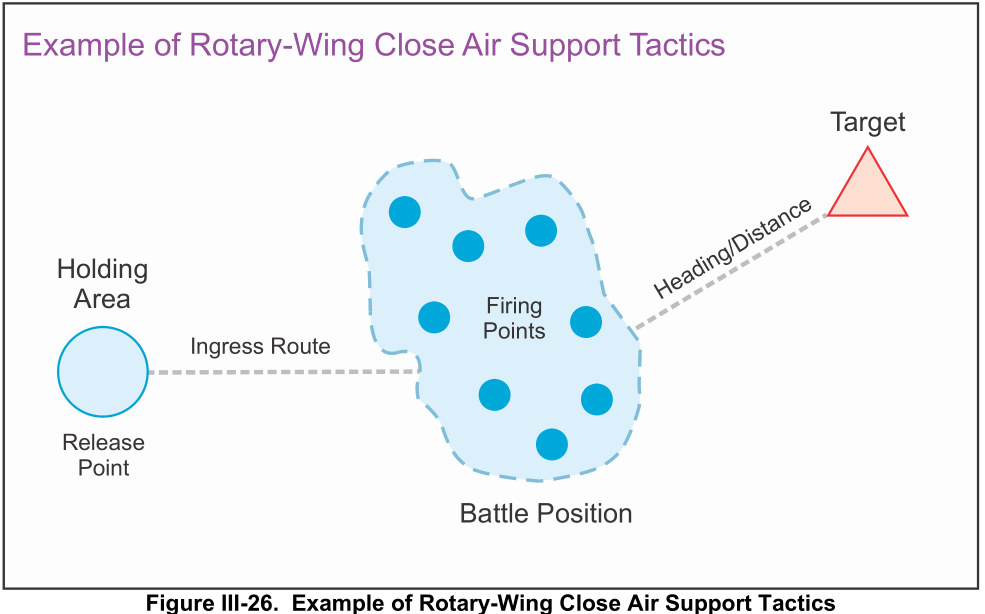
\includegraphics[width=\textwidth]{attackphase.png}
    \caption{Phase d'attaque.}
    \label{fig:attackphase}
\end{figure}

\subsection{Techniques de mouvement}

\e
    \item Du fait de la proximité de la menace, les \glspl{rw} utilisent le terrain pour se déplacer vers la \gls{bp}.
    \item Il existe 3 techniques de mouvement:
    \ee
        \itemt{Travelling}{Le travelling est utilisé lorsque le contact avec l’ennemi est peu probable. La formation dans son ensemble progresse en suivant le terrain, avec des secteurs de scanning prédéfinis. Ce mode de déplacement permet une vitesse élevée dans des zones relativement sécurisées.}
        \itemt{Travelling overwatch}{Le travelling overwatch est utilisé lorsque le contact avec l’ennemi est possible. La formation se déplace en vol de contour ou en vol NOE, avec un élément de tête en évolution constante et un élément de surveillance en retrait, qui se repositionne de manière à fournir un appui visuel et armé constant à l’élément de tête. Ce mode de déplacement lorsque la prudence est de mise mais la vitesse reste souhaitable.}
        \itemt{Bounding Overwatch}{Le bounding overwatch est utilisé lorsque le contact avec l’ennemi est imminent. La formation se déplace en vol NOE, et est divisée en deux éléments, qui se déplacent alternativement, l’élément statique fournissant une couverture visuelle et armée constante à l’élément en mouvement à partir d’une position protégée.}
    \ed
\ed

\subsubsection{Résumé des types de mouvements}

\e
    \item Extrait du \jp:\\
    \begin{figure}[H]
        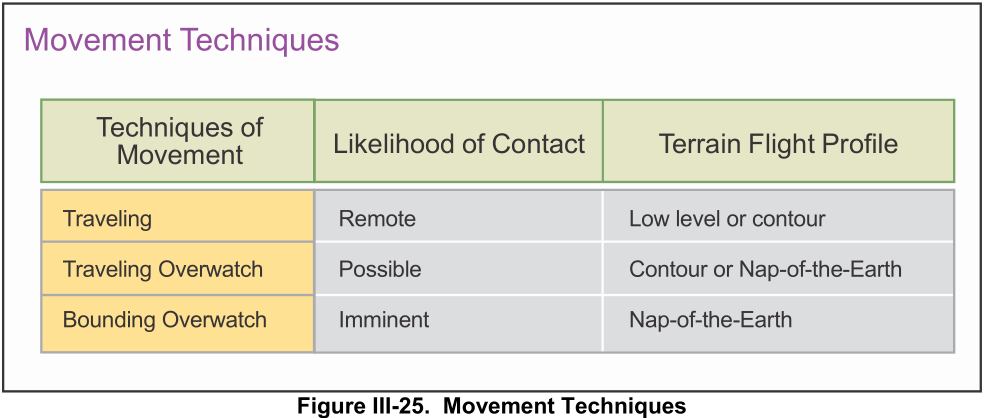
\includegraphics[width=\textwidth]{movementtypes.png}
        \caption{Types de mouvements pour les unités \gls{rw}.}
        \label{fig:movementtypes}
    \end{figure}
\ed

\subsubsection{Communications et contrôle}

\e
    \item
    Généralement, pendant la phase de pénétration, il sera préférable que la patrouille assure d’abord sa sécurité, ce qui peut entraîner une perte des communications de par la faible altitude nécessaire.
    \item La patrouille sera alors entièrement briefée avant de quitter la HA, et les communications reprendront une fois établi à la BP.
    \item Un relais aérien peut également être mis en place.
\ed

\section{Phase d’attaque}

\subsection{Contrôle}

\e
    \item Une fois la BP atteinte, le \gls{jtac}/\gls{faca} donnera les instructions finales à la patrouille.
    \item Les membres de la patrouilles choisissent leurs positions de tir, et restent masqués en attendant le \gls{tot}/\gls{ttt} ou l’ordre d’attaque
\ed

\subsection{Attaque}

\e
    \item Il existe 3 profils d’attaque: le tir stationnaire, le tir en route, et le tir plongeant.
\ed

\subsubsection{Tir stationnaire}

\e
    \item
    Le tir stationnaire s’effectue après un pop-up ou un stand-off, en vol stationnaire ou en vol vers l'avant très lent. \textbf{L’appareil doit rester stationnaire le moins longtemps possible}, et se repositionner une fois le tir effectué.
    \item
    Ce type de tir est le plus efficace pour délivrer les munitions guidées (Vikhrs). Le tir de munitions non guidée depuis le vol stationnaire c’est pas recommandé, car l’hélicoptère à une tendance à l’instabilité plus prononcée en vol stationnaire.
\ed

\subsubsection{Tir en route}

\e
    \item Le tir en route consiste à tirer les munitions en déplacement vers l’avant à altitude constante. Ce tir permet une plus grande stabilité de la plate-forme.
    \item
    Le tir en route permet de réduire la vulnérabilité de l’hélicoptère au tir d’armes de petit calibre, et améliore la capacité de réponse à un tir d’arme air-sol guidée contre l’hélicoptère de par l’énergie déjà acquise.
\ed

\subsubsection{Tir plongeant}

\e
    \item
    Le tir plongeant est effectué en déplacement vers l’avant et en descente, offre une précision accrue lors du tir de munitions non guidée, et permet à l’appareil de rester hors de l’enveloppe de tir des armes de petit calibre.

    \item
    La position élevée permet également une \gls{sa} très élevée, de par l’altitude plus importante. Cependant, cela implique une grande vulnérabilité aux missiles infrarouges.
\ed

\subsection{Désengagement et egress}

\e
    \item
    Une fois les actions nécessaires effectuées, ou lorsque le “play time” est écoulé, \textbf{le chef de patrouille devra effectuer un check-out avec le \gls{jtac}/\gls{faca}}, et quitter la zone via une route planifiée ou assignée.
    \item Les considération sur le retour sont identiques à celles de l’aller.
    \item Les \gls{rw}s peuvent utiliser un FARP pour le rearm/refuel, et ainsi allonger le temps pendant lequel ils sont à même de soutenir les troupes au sol alliées.
    \item \important{Lorsque la mission se termine, le chef de patrouille devra fournir un \gls{bda} et un \gls{misrep} au \gls{cc}.}

\ed







\chapter*{Remerciements}
\phantomsection
\addcontentsline{toc}{chapter}{\protect\numberline{}Remerciements}

Un grand merci à la \onethreetwo{}, qui m'a initié au Close Air Support, et qui invite régulièrement la \thirdwing{} à ses événements bluffants de réalisme.

Merci à eux également pour m'avoir autorisé à inclure leurs GRGs dans ce document à titre d'exemple.

\newpage

\pagenumbering{Roman}

\phantomsection
%\addcontentsline{toc}{chapter}{\listfigurename}
\addtocontents{lof}{\protect\addcontentsline{toc}{chapter}{Liste des images}}
\listoffigures

\newpage

\phantomsection
%\addcontentsline{toc}{chapter}{\listtablename}
\addtocontents{lot}{\protect\addcontentsline{toc}{chapter}{Liste des tables}}
\listoftables

\newpage

\phantomsection
%\addcontentsline{toc}{chapter}{\lstlistlistingname}
\addtocontents{lol}{\protect\addcontentsline{toc}{chapter}{Liste des exemples}}
\lstlistoflistings{}

\newpage

\glossarystyle{altlist}
\printglossary[title=Glossaire, toctitle=Glossaire, type=main]

\newpage
\printglossary[title=Acronymes, toctitle=Acronymes, type=\acronymtype]

%\clearpage
%\phantomsection
%\addcontentsline{toc}{section}{Bibliographie}

\begin{appendices}
	
    \chapter{Guide de préparation de mission}\label[annex]{ann1}

\e
    \item Situation alliée
    \ee
        \item FLOT
        \item Points remarquables
        \eee
            \item Points de contact
            \item Points de rapportages
            \item Points initiaux
        \ed
        \item Dispositif allié
        \eee
            \item Zone d’opération
            \item Type de terrain
            \item Position et callsigns du J-TAC/FAC(A)
            \item Unités alliées en support
        \ed
        \item Contrôle et coordination
        \eee
            \item Mesures permissives
            \item Mesures restrictives
        \ed
        \item Gestion de l’espace aérien
        \item Zones d’engagement de la chasse
    \ed
    \item Situation ennemie
    \ee
        \item Position et force de l’ennemi
        \eee
            \item Intention supposée
            \item Route de déplacement probable
            \item Tactiques déjà observées
        \ed
        \item Éléments de support ennemis
        \item Menaces
        \eee
            \item Position
            \item Type de guidage
            \eeee
                \item Infrarouge
                \item Radar
                \item Optique
            \ed
            \item Capacité de la menace (portée, puissance)
            \item Éléments révélateurs
            \item Tactiques déjà observées
        \ed
    \ed
    \item Météo
    \ee
        \item Plafond
        \item Visibilité
        \item Température
        \item Vent
    \ed
    \item Environnement
    \ee
        \item Élévation et azimuth du soleil
        \item Lever et coucher du soleil
    \ed
    \item Objectifs de mission
    \ee
        \item Objectifs globaux de l’opération
        \item Objectifs du haut commandement
        \item Objectifs de la sortie
        \item Objectifs des unités alliées
        \item Ordre de priorité des différentes cibles potentielles
        \item Heure d’arrivée prévue/imposée sur objectif
        \item Règles d’engagement
    \ed
\ed





    
    \chapter{Carte de mission}\label[annex]{ann2}


\renewcommand{\arraystretch}{3.7}
\setlength{\extrarowheight}{-25pt}
{\footnotesize
\begin{tabularx}{\textwidth}{ @{} X @{} }

	{\begin{tabularx}{\textwidth}{@{} X X @{}}
		\textbf{Mission} & Date
	\end{tabularx}}\\ \midrule
	
	\multicolumn{1}{c}{\textbf{Wx}}\\[-3ex] \midrule
	{\begin{tabularx}{\textwidth}{@{} *{7}X @{}}
		Vis & Ceil & Cov & Wind & QNH & Temp & ATIS
	\end{tabularx}}\\ \midrule
	
	{\begin{tabularx}{\textwidth}{@{} X | X @{}}
		{\begin{tabularx}{\linewidth}{@{} X X @{}}
			\multicolumn{2}{c}{\textbf{Fuel}}\\[-3ex] \midrule
			Joker & Bingo\\
		\end{tabularx}} &
		{\begin{tabularx}{\linewidth}{@{} X X @{}}
			\multicolumn{2}{c}{\textbf{Loadout}}\\[-3ex] \midrule
			Int & Ext\\
		\end{tabularx}}
	\end{tabularx}}\\ \midrule
	
	\multicolumn{1}{c}{\textbf{Dep/Rec}}\\[-3ex] \midrule
	{\begin{tabularx}{\textwidth}{@{} *{7}X @{}}
		Airbase & Gnd & Twr & App & Lat & Long & Remarks\\[-3ex] \midrule
		\hfill & \hfill & \hfill & \hfill & \hfill & \hfill & \hfill\\ \midrule
		\hfill & \hfill & \hfill & \hfill & \hfill & \hfill & \hfill\\ \midrule
		\hfill & \hfill & \hfill & \hfill & \hfill & \hfill & \hfill\\
	\end{tabularx}}\\ \midrule
	
	\multicolumn{1}{c}{\textbf{Comms}}\\[-3ex] \midrule
	{\begin{tabularx}{\textwidth}{@{} *{2}X @{}}
		Pri & Sec\\[-3ex]
	\end{tabularx}}\\ \midrule
	{\begin{tabularx}{\textwidth}{@{} X | X @{}}
		{\begin{tabularx}{\linewidth}{@{} *{3}X @{}}
			Callsign & Role & Freq\\[-3ex] \midrule
			\hfill & \hfill & \hfill\\ \midrule
			\hfill & \hfill & \hfill\\ \midrule
			\hfill & \hfill & \hfill\\ \midrule
			\hfill & \hfill & \hfill\\
		\end{tabularx}} &
		{\begin{tabularx}{\linewidth}{@{} *{3}X @{}}
			Callsign & Role & Freq\\[-3ex] \midrule	
			\hfill & \hfill & \hfill\\ \midrule
			\hfill & \hfill & \hfill\\ \midrule
			\hfill & \hfill & \hfill\\ \midrule
			\hfill & \hfill & \hfill\\
		\end{tabularx}}\\
	\end{tabularx}}\\ \midrule
	
	\multicolumn{1}{c}{\textbf{Points}}\\[-3ex] \midrule
	{\begin{tabularx}{\textwidth}{@{} X | X @{}}
		{\begin{tabularx}{\linewidth}{@{} *{4}X @{}}
			Nom & Action & Lat & Long\\[-3ex] \midrule
			\hfill & \hfill & \hfill & \hfill\\ \midrule
			\hfill & \hfill & \hfill & \hfill\\ \midrule
			\hfill & \hfill & \hfill & \hfill\\ \midrule
			\hfill & \hfill & \hfill & \hfill\\ \midrule
			\hfill & \hfill & \hfill & \hfill\\ \midrule
			\hfill & \hfill & \hfill & \hfill\\
		\end{tabularx}} &
		{\begin{tabularx}{\linewidth}{@{} *{4}X @{}}
			Nom & Action & Lat & Long\\[-3ex] \midrule
			\hfill & \hfill & \hfill & \hfill\\ \midrule
			\hfill & \hfill & \hfill & \hfill\\ \midrule
			\hfill & \hfill & \hfill & \hfill\\ \midrule
			\hfill & \hfill & \hfill & \hfill\\ \midrule
			\hfill & \hfill & \hfill & \hfill\\ \midrule
			\hfill & \hfill & \hfill & \hfill\\
		\end{tabularx}}\\
	\end{tabularx}}\\ \midrule
	{\begin{tabularx}{\textwidth}{@{} p{4cm} | X @{}}
		\begin{tabular}[t]{@{} l @{}}
			\multicolumn{1}{c}{\textbf{FENCE IN}}\\[-3ex] \midrule
			Fuel\\[-3ex]
			Emitters\\[-3ex]
			Navigation\\[-3ex]
			Communications\\[-3ex]
			ECM\\[-3ex]
			\midrule
			\multicolumn{1}{c}{\textbf{Menaces}}\\[-3ex] \midrule
			{\begin{tabularx}{\linewidth}{@{} r X X @{}}
				SA18 & 5k & 3k\\[-3ex] \midrule
				SA9 & 4.2k & 3.5k\\[-3ex] \midrule
				SA13 & 5k & 3.5k\\[-3ex] \midrule
				ZU23 & 2.5k & 2k\\[-3ex] \midrule
				Shilka & 2.5k & 2k\\[-3ex] \midrule
			\end{tabularx}}
		\end{tabular} &
		\textbf{Remarques}\\
	\end{tabularx}}\\
\end{tabularx}
}
%}




\end{appendices}


\end{document} 